\documentclass[a4paper,14pt,oneside,openany]{memoir}
\usepackage[left=2.5cm, right=1cm, top=2cm, bottom=2cm]{geometry}

\usepackage[backend=biber,style=numeric,sorting=none]{biblatex}
\DeclareFieldFormat{labelnumberwidth}{{#1\adddot}}

\usepackage{bm}
\usepackage{amsmath}
\usepackage[russian]{babel}
\renewcommand{\baselinestretch}{1.5}
\setlength{\parindent}{1.25cm}
\usepackage{indentfirst}
\usepackage[utf8]{inputenc}
\usepackage{csquotes}
\usepackage{verbatim} % multi comments

%% pics, tables
\usepackage{graphicx}
\usepackage{caption}
\captionsetup[figure]{name={Рисунок}, labelsep={space}}
\captionsetup[table]{labelsep={space}}
\graphicspath{ {./pics/lims/} {./pics/mau/}, {./pics/observer/}, {./pics/acsl/}, {./pics/}}
\usepackage{subfig}

%% sections style
\usepackage{titlesec}
\titleformat*{\section}{\normalfont\bfseries}

%% page style
\pagestyle{myheadings} % нумерация страниц вверху справа
\aliaspagestyle{chapter}{myheadings} % нумерация страниц вверху справа
\renewcommand{\cftchapterpagefont}{\normalfont}% нежирные номера страниц у глав в оглавлении
\renewcommand{\cftchapterleader}{\cftdotfill{\cftchapterdotsep}}% нежирные точки до номеров страниц у глав в оглавлении
\renewcommand{\cftchapterfont}{}% нежирные названия глав в оглавлении

\addbibresource{bibliography/citations.bib}

\begin{document}
	\thispagestyle{empty}
\begin{center} 
«Федеральное государственное автономное образовательное учреждение высшего образования «Московский физико-технический институт (национальный исследовательский университет)»
\end{center}
\begin{center} 
Физтех-школа Аэрокосмических Технологий
\end{center}

{
   	\vskip 5mm
}

\begin{flushleft}
\textbf{Направление подготовки:} 24.06.01 Авиационная и ракетно-космическая техника

\textbf{Направленность (профиль) подготовки:} 05.07.09 Динамика, баллистика, управление движением летательных аппаратов

\textbf{Форма обучения:} очная
\end{flushleft}

{
	\vskip 1cm
}

\begin{center} 
\textbf{НАУЧНЫЙ ДОКЛАД ОБ ОСНОВНЫХ РЕЗУЛЬТАТАХ ПОДГОТОВЛЕННОЙ НАУЧНО-КВАЛИФИКАЦИОННОЙ РАБОТЫ (ДИССЕРТАЦИИ)}
\end{center}

\begin{center} 
\textbf{«Анализ динамики и разработка методов управления движением квадрокоптера с поворотными роторами»}
\end{center}

{
	\vskip 1cm
}


\begin{flushright}
\textbf{Aспирант:} Шавин Михаил Юрьевич \hspace{16mm} \vspace{5mm}

$\rule{5cm}{0.15mm}$

\textbf{Научный руководитель:}  \hspace{41mm}

Притыкин Дмитрий Аркадьевич, к.ф.-м.н., \hspace{6mm} 

ст. науч. сотр. Космического центра Сколтеха \vspace{5mm}

$\rule{5cm}{0.15mm}$

\end{flushright}

{
	\vskip 5mm
}

\begin{center} 
Москва 2019
\end{center}

	\tableofcontents
	
\chapter{Общая характеристика научного доклада}

\section{Актуальность темы исследования}

Беспилотные летательные аппараты (БЛА) мультироторного типа находят всё более широкое применение в различных областях человеческой деятельности, а миниатюризация и доступность электронных компонентов их бортового оборудования приводит к расширению спектра задач, в решении которых используются такие аппараты.
Интерес исследователей к БЛА обусловлен также и тем, что они являются доступным средством для отработки новых технологий в аэрокосмической отрасли \cite{Otero01}.
С момента создания первых квадрокоптеров интенсивно ведутся исследования в области их динамики и управления, причём количество работ растет с каждым годом, что можно наблюдать по динамике количества публикаций (рис. \ref{pic:res_amount}), посвященных квадрокоптерам, доступных на крупнейшей онлайн платформе научных публикаций «Google Академия».
Однако, несмотря на обилие публикаций, в области управляемой динамики квадрокоптеров остаются перспективные направления, среди которых усовершенствование конструкции БЛА, связанное с увеличением размерности вектора управляющих воздействий.
Конструктивно это достигается, например, с помощью сервоприводов, способных поворачивать роторы с пропеллерами относительно корпуса.
\begin{figure}[h!]
	\centering
	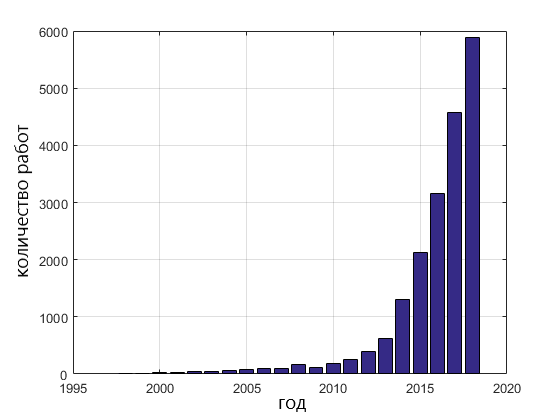
\includegraphics[width=0.95\columnwidth]{res_amount}
	\caption{ -- Динамика количества публикаций, посвященных квадрокоптерам}
	\label{pic:res_amount}
\end{figure}

Стандартный квадрокоптер с четырёхмерным вектором управляющих воздействий и шестью степенями свободы корпуса аппарата не способен, например, независимо управлять положением и ориентацией.
Это приводит к необходимости дополнительных устройств для наведения камер или лазерных дальномеров, используемых при выполнении ряда стандартных для БЛА задач.
Возможность независимо управлять положением и ориентацией, приобретаемая за счёт использования поворотных роторов, влияет не только на работу полезной нагрузки и датчиков, но и на функциональные возможности всей системы в целом.
Согласно работе \cite{Stolc01} усовершенствованные таким образом квадрокоптеры более устойчивы к возмущениям внешней среды, а также лучше стандартных квадрокоптеров пригодны для вертикального взлёта и посадки на неровные поверхности.
Достоинства БЛА с поворотными роторами отмечают и исследователи, работающие над управлением БЛА в экстренных ситуациях (при отказе части двигателей) \cite{Morozov01, Shidar00}.
В работе \cite{Shidar00} обосновывается достижение более высокой скорости за счёт выбора оптимальной по отношению к набегающему потоку ориентации, а также более рациональное по сравнению со стандартными аппаратами энергопотребление.
В работе \cite{Morozov01} отмечена перспективность конструкции с поворотными роторами, однако её применение не рассматривается из-за сложности реализации.
Использование поворотных роторов действительно усложняет реализацию контура управления \cite{Ryll01, Falconi01, Segui01, Oosedo01} и не позволяет применять ставшую классической изящную схему управления \cite{Mellinger01}, однако, есть основания полагать, что предлагаемое в данной работе аналитическое обращение динамики системы позволит преодолеть некоторую часть возникающих трудностей.

\section{Цели и задачи исследования}

Объектом исследования является система управления движением квадрокоптера с поворотными роторами, предметом исследования -- динамика и методы управления движением квадрокоптера с поворотными роторами.

Цель работы -- выполнить анализ динамики квадрокоптера с поворотными роторами;
разработать алгоритмы управления движением квадрокоптера с поворотными роторами для выполнения различных манёвров; разработать алгоритмы управления движением квадрокоптера с поворотными роторами для экстренного сценария -- потере двух смежных двигателей. Для достижения цели работы необходимо решить следующие задачи:
\begin{enumerate}
	\item Разработать математическую модель движения квадрокоптера с поворотными роторами с учётом сил и моментов, действующих на все составные части системы.
	\item Решить задачу обратной динамики и синтезировать контур управления квадрокоптером с поворотными роторами для независимого управления положением и ориентацией аппарата с учётом физических ограничений, накладываемых на исполнительные органы системы управления.
	\item Обеспечить обратную связь в контуре управления, реализовать алгоритмы оценки состояния на основе фильтра Калмана.
	\item Реализовать в синтезированном контуре алгоритм управления положением и ориентацией аппарата, позволяющий совершать сложные манёвры, как, например, отслеживание подвижного объекта с помощью жестко закрепленной бортовой камеры.
	\item Реализовать алгоритмы управления квадрокоптером с поворотными роторами в случае отказа двух смежных двигателей, позволяющие аппарату выполнение номинальных задач.
\end{enumerate}
Для решения сформулированных задач используются классические методы механики, управления, вычислительной и высшей математики.

Область данного исследования соответствует пунктам «Баллистическое проектирование летательных аппаратов различного назначения» и «Динамическое проектирование управляемых летательных аппаратов и исследование динамики их движения» паспорта специальности «05.07.09 – Динамика, баллистика, управление движением летательных аппаратов».

\section{Положения, выносимые на публичное представление}
Положения, выносимые на публичное представление:
\begin{enumerate}
\item Математическая модель управляемой динамики квадрокоптера с поворотными роторами с учётом сил и моментов, действующих на все составные части системы;
\item Синтез контура управления квадрокоптером с поворотными роторами для независимого управления положением и ориентацией; 
\item Алгоритм для учёта физических ограничений, накладываемых на исполнительные органы системы управления;
\item Алгоритм идентификации аэродинамических параметров пропеллеров;
\item Алгоритмы экстренного управления квадрокоптером с поворотными роторами в случае отказа двух смежных двигателей.
\item Выводы и рекомендации, сформулированные в работе.
\end{enumerate}

\section{Степень достоверности и апробация результатов}
Достоверность полученных научных положений, результатов и выводов обеспечивается
соответствием выбранных моделей движения общепринятым стандартам,
адекватностью выбранных методов исследования движения,
проведением численного моделирования полученных аналитических результатов,
а также сопоставлением с результатами,
полученными другими авторами для частных случаев рассматриваемых задач.

Основные научные положения и результаты работы докладывались и обсуждались на 
\begin{itemize}
\item Всероссийской конференции молодых ученых-механиков, 5 - 15 сентября 2017 г., г. Сочи, «Буревестник» МГУ;
\item Международной научной конференции «Фундаментальные и прикладные задачи механики», 24 - 27 октября 2017 г., г. Москва;
\item 60-й Всероссийской научной конференции МФТИ, секция теоретической механики, 20–26 ноября 2017 г., г. Долгопрудный;
\item 60-й Всероссийской научной конференции МФТИ, секция управления динамическими системами, 20–26 ноября 2017 г., г. Москва;
\item седьмой международной конференции «Geometry, Dynamics, Integrable Systems», 5-9 июня 2018 г., г. Москва;
\item XIV Международной конференции «Устойчивость и колебания нелинейных систем управления» (конференция Пятницкого) Россия, Москва, ИПУ РАН, 30 мая -- 1 июня 2018 г.
\item 14-ой международной конференции «Vibration engineering and technology of machinery», 10-13 сентября 2018 г., г. Лиссабон, Португалия;
\item Международной конференции «Проблемы механики и управления», 16-22 сентября 2018 г., г. Махачкала;
\item XXI конференции молодых ученых «Навигация и управление движением», 19–22 марта 2019 г., г. Санкт-Петербург.
\end{itemize}
По теме исследования были опубликованы 10 работ, список можно найти на странице \pageref{list_chapter}.

\section{Научная новизна и практическая значимость работы}
Научная новизна представленных в диссертации результатов заключается в следующем:
\begin{enumerate}
	\item  Получено аналитическое решение задачи обратной динамики БЛА с поворотными роторами;
	\item  Проведен анализ аналитического решения задачи обратной динамики  БЛА с поворотными роторами, разработан алгоритм реализации ограничений на компоненты вектора управляющих воздействий;
	\item  Разработаны алгоритмы экстренного управления квадрокоптером с поворотными роторами в случае отказа двух смежных двигателей.
\end{enumerate}

Практическая значимость работы состоит в том, что
реализация разработанной в исследовании системы управления позволяет проектировать БЛА с улучшенными относительно стандартных квадрокоптеров лётными характеристиками, в том числе обладающих способностью 
выполнять сложные манёвры, недоступные стандартным квадрокоптерам, такие, как манёвры с требованием независимого управления положением и ориентацией.
Таким образом, расширяются возможности беспилотных летательных аппаратов.
Кроме этого, реализованная в программных алгоритмах динамическая модель и система управления позволяет на предварительном этапе проектирования БЛА определить параметры регулятора и динамики мультироторного робота в зависимости от выбранных комплектующих и других факторов.

\section{Личный вклад автора}
Все результаты, вынесенные на защиту, получены автором самостоятельно.
Также автором самостоятельно проведены численные эксперименты,
подтверждающие основные положения и выводы работы. 












	
\chapter{Управляемая динамика квадрокоптера с поворотными роторами}

\section{Основные элементы конструкции квадрокоптера с поворотными роторами}

Основным элементом конструкции БЛА является корпус, из которого выходят лучи с закрепленными на концах двигателями с пропеллерами. Лучи расположены симметрично относительно корпуса аппарата и реализуют так называемую Х-схему. Смежные пропеллеры имеют противоположное направление вращения; первый и третий – пропеллеры левого вращения, а второй и четвертый – правого. Каждый из роторов может поворачиваться посредством сервопривода вокруг продольной оси луча, на котором он закреплен. Для построения математической модели динамики БЛА условимся, что он сконструирован таким образом, что
\begin{itemize}
	\item главные центральные оси инерции аппарата и каждого из роторов совпадают с осями симметрии; 
	\item корпус БЛА и каждый из четырех роторов являются твердыми телами; 
	\item под ротором будем понимать вращающуюся часть двигателя и пропеллер, которые являются одним телом; 
	\item крепление роторов к корпусу БЛА происходит в точке, совпадающей с центрами масс роторов, помимо роторов с пропеллерами в системе отсутствуют подвижные части;
	\item центры масс роторов лежат на окружности радиуса $L$, центр окружности совпадает с центром масс корпуса аппарата.
\end{itemize}
Общий вид аппарата представлен на рисунке \ref{fig:tiltrotor_scheme}.

\section{Постановка задачи управления}
\label{section_ctrl_task}

Считая заданной требуемую траекторию БЛА в координатном пространстве, положим целью управления обеспечение наперёд заданной траектории центра масс аппарата, а также требуемой ориентации. Такая постановка позволяет формализовать следующие задачи:
\begin{itemize}
\item приведение центра масс БЛА в некоторое наперёд заданное статичное положение;
\item стабилизация ориентации БЛА относительно некоторого наперёд заданного положения;
\item перемещение центра масс БЛА вдоль некоторой наперёд заданной (дискретным набором точек или как непрерывная функция координат от времени) траектории;
\item слежение за объектом, перемещающимся произвольным образом;
\item наведение камеры, установленной на БЛА на неподвижный или перемещающийся объект (то есть съёмка неподвижного объекта с разных ракурсов или слежение камерой за подвижным объектом).
\end{itemize}

Решение последней задачи в явном виде использует степени свободы, связанные с увеличением размерности вектора управляющих параметров. Стоит отметить, что квадрокоптер со стандартной конструкцией произвольный маневр наведения камеры в точку с одновременным изменением высоты выполнить не способен.
\begin{figure}[h]
	\centering
	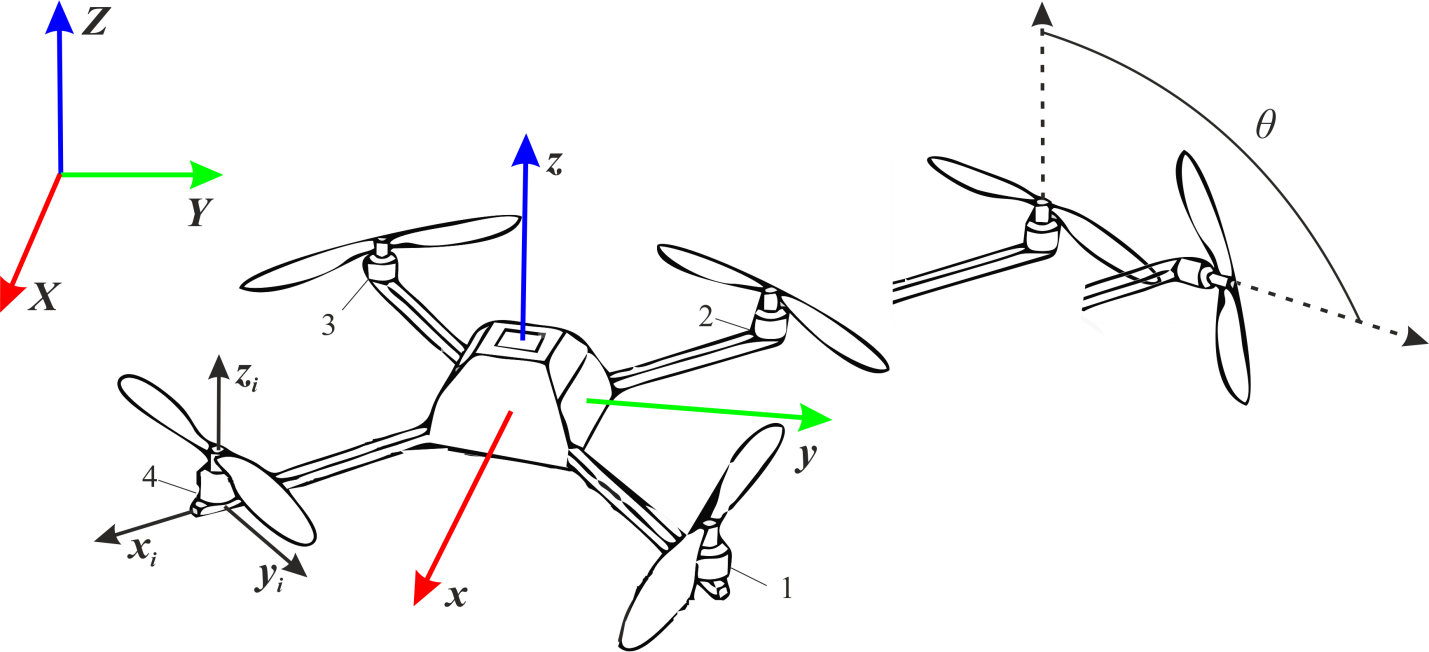
\includegraphics[scale=0.9]{tiltrotor_scheme}
	\caption{ -- Общая схема квадрокоптера с поворотными роторами}
	\label{fig:tiltrotor_scheme}
\end{figure}

\section{Математическая модель динамики БЛА}

Движение аппарата рассматривается относительно неподвижной инерциальной системы отсчета $I$, связанной с Землей (вращением Земли на характерных временах автономного полёта БЛА рассматриваемого класса принято пренебрегать).
Направление осей выбрано по схеме «Восток, Север, Верх» (ENU) -- ось \textbf{$X_I$} направлена на восток, ось \textbf{$Y_I$} -- на север, а ось \textbf{$Z_I$} -- от центра Земли.

Индексом $B$ обозначим жестко связанную с корпусом аппарата систему координат с началом в центре масс и осями, совпадающими с главными центральными осями инерции корпуса БЛА.
Для промежуточных выкладок нами будет использована ещё одна жестко связанная с корпусом система координат $B'$, полученная из $B$ поворотом вокруг оси $Z_B$ таким образом, что ось $X_B'$ направлена вдоль луча, несущего первый ротор согласно схеме \ref{fig:tiltrotor_scheme}.

Индексами $R_i$ будем обозначать системы координат, жестко связанные с роторами и совпадающие с их главными центральными осями инерции.

При записи векторов будем отмечать верхним индексом систему координат, в которой записано разложение вектора. Повороты систем координат друг относительно друга будем описывать кватернионами. Будем говорить, что кватернион $q_{IB}$ задаёт ориентацию системы координат $B$ относительно $I$ в том смысле, что разложения некоторого вектора $\bm{r}$ в этих двух базисах связаны соотношением
\begin{equation} \label{eq:m_quat}
\bm{r}^I = q_{IB} \circ \bm{r}^B \circ \tilde{q}_{IB}.
\end{equation}

Положение БЛА в пространстве определяется радиус-вектором его центра масс $\bm{r}^I$ и кватернионом ориентации $q_{IB}$. Скорость центра масс аппарата равна
\begin{equation} \label{eq:m_vel}
\bm{v}^I = \dot{\bm{r}^I}.
\end{equation}
Изменение кватерниона ориентации аппарата определяется уравнением Пуассона
\begin{equation} \label{eq:m_puasson}
\dot{q}_{IB} = \frac{1}{2} {q}_{IB} \circ \bm{\Omega}^B,
\end{equation}
где $\bm{\Omega}_B$ – угловая скорость корпуса БЛА в проекции на собственные оси.

Движение центра масс БЛА определяется уравнением
\begin{equation} \label{eq:m_traslational_motion}
\ddot{\bm{r}} = M \bm{g}^I - \frac{1}{2} \rho C S_{\perp} |\bm{v}^I| \bm{v}^I + \sum_{i=1}^{4}{ { (-1)^{i+1} k \tilde \omega_i |\tilde \omega_i| \bm{e}^I_{z_i}}},
\end{equation}
где три члена в правой части соответствуют силе тяжести, силе аэродинамического сопротивления и создаваемой пропеллерами тяге, $M = m + \sum_{i=1}^{4}{m_i}$ – общая масса корпуса, $m_i$ – масса $i$-го ротора с пропеллером, $\bm g$ – ускорение свободного падения, $S_{\perp}$ – площадь миделева сечения корпуса аппарата, $C$ – аэродинамический коэффициент сопротивления воздуха, $\bm{e}^I_{z_i}$ – единичный вектор вдоль оси симметрии i-го ротора, $k$ – аэродинамический коэффициент, определяемый экспериментально; $\tilde \omega_i$ – скорость вращения i-го пропеллера.

Для описания вращательного движения воспользуемся динамическими уравнениям Эйлера
\begin{equation} \label{eq:m_rotational_motion}
\bm{\tau}^{B} =
\bm{J}_B\dot{\bm{\Omega}}^B + \bm{\Omega}^B \times \bm{J}_B{\bm{\Omega}^B},
\end{equation}
где $\bm{J}_B$ — тензор инерции корпуса в главных осях корпуса; $\bm{\tau}^{B}$ —
главный момент сил, действующий на корпус.

Главный момент сил складывается из моментов сил, действующих на корпус аппарата со стороны поворотных роторов с пропеллерами и внешних моментов:
\begin{equation} \label{eq:m_general_torq}
\bm{\tau}^{B} =
-\sum_{i=1}^{4} {\bm{\tau}^{B}_i} +
\sum_{i=1}^{4} {\bm{r}^B_i \times (-1)^{i+1} k \tilde \omega_i |\tilde \omega_i| \bm{e}^I_{z_i},}
\end{equation}
где $\bm{\tau}^{B}_i$ — моменты сил, действующие на роторы со стороны аппарата, $\bm{r}^B_i$ -- радиус-вектор, проведенный из центра масс квадрокоптера $i$-тому к ротору. Вычислим угловую скорость $i$-го ротора в проекциях на оси $R_i$:
\begin{equation} \label{eq:m_prop_ang_vel}
\bm{\omega}^{R_i}_i =
q_{{R_i} B} \circ (\bm{\Omega}^B + \dot {\theta}_i \bm e^B_{r_i}) \circ \tilde {q}_{{R_i}B} +
\tilde \omega_i \bm{e}^{R_i}_{z_i},
\end{equation}
где $\bm e^B_{r_i}$ -- орт вектора $\bm{r}^B_i$, ${\theta}_i$ -- угол поворота $i$-того ротора. Запишем динамические уравнения Эйлера для роторов.
\begin{equation} \label{eq:m_rotors_dyn}
\bm{\tau}^{{R_i}}_i + \bm{\varsigma}^{{R_i}}_{i} = 
\bm{J}_{R_i}\dot{\bm{\omega}}^{R_i}_i + \bm{\omega}^{R_i}_i \times \bm{J}_{R_i}{\bm{\omega}^{R_i}_i},
\end{equation}
где $\bm{J}_{R_i}$ -- тензор инерции $i$-того ротора с пропеллером, записанный в собственных главных осях, $\bm{\varsigma}^{{R_i}}_{i}$ -- внешний момент силы, для которого запишем:
\begin{equation} \label{eq:m_ext_torq}
\begin{aligned}
&\bm{\varsigma}^{{R_i}}_{i} = -b \tilde \omega_i |\tilde \omega_i| \bm e^{R_i}_{r_i}\\
&\bm{\varsigma}^{B}_{i} = q_{ B {R_i}} \circ \bm{\varsigma}^{{R_i}}_{i} \circ \tilde q_{ B {R_i}}.
\end{aligned}
\end{equation}
Здесь $b$ -- аэродинамический коэффициент, определяемый экспериментально.

Окончательно уравнения вращательной динамики аппарата принимают вид:
\begin{equation} \label{eq:m_final_rotational_motion}
\begin{aligned}
\bm{J}_B\dot{\bm{\Omega}}^B + \bm{\Omega}^B \times \bm{J}_B{\bm{\Omega}^B} =
&\sum_{i=1}^{4} {\bm{r}^B_i \times
	(-1)^{i+1} k \tilde \omega_i |\tilde \omega_i| \bm{e}^I_{z_i}} + \\ +
\sum_{i=1}^{4} {\bm{\varsigma}^{{R_i}}_{i}} +
&\sum_{i=1}^{4} q_{ B {R_i}} \circ (\bm{J}_{R_i}\dot{\bm{\omega}}^{R_i}_i + \bm{\omega}^{R_i}_i \times \bm{J}_{R_i}{\bm{\omega}^{R_i}_i}) \circ \tilde q_{ B {R_i}}
\end{aligned}
\end{equation}
Уравнения (\ref{eq:m_vel}), (\ref{eq:m_puasson}), (\ref{eq:m_traslational_motion}) и (\ref{eq:m_final_rotational_motion}) составляют замкнутую систему, позволяющую моделировать динамику полета квадрокоптера с поворотными роторами.

\section{Синтез регулятора}

Пусть задана требуемая траектория центра масс аппарата $\bm r^0(t)$, а также требуемая ориентация $q^0(t)$. Обозначим  $\delta \bm r(t) = \bm r^0(t) - \bm r(t)$ и $\delta q(t) = q^0(t) \circ \tilde q(t)$, где $\delta \bm r$ и $\delta q$ определяют расхождение требуемой и текущей траектории БЛА в координатном пространстве, а $q = q_{IB}$.  В качестве переменных управления выберем скорости вращения пропеллеров ${\tilde \omega}_i$ и углы поворота роторов ${\theta}_i$:
\begin{equation} \label{eq:m_ctrl_out}
\begin{aligned}
	&\bm{u} = (\bm \omega_u, \bm \theta_u)^T,
	\\
	\bm \omega_u =
	(\tilde\omega_1 |\tilde\omega_1|,
	\tilde\omega_2 |\tilde\omega_2|&,
	\tilde\omega_3 |\tilde\omega_3|,
	\tilde\omega_4 |\tilde\omega_4|)^T,
	\quad
	\bm \theta_u = (\theta_1, \theta_2 , \theta_3 , \theta_4 )^T.
\end{aligned}
\end{equation}
Регуляторы, обеспечивающие необходимое управление по положению и ориентации могут быть построены, как
\begin{equation} \label{eq:m_reg}
\begin{aligned}
	\ddot{\bm{r}_d}(t)&=
	\ddot{\bm{r}}^0(t)+\bm{K}_{r1}(\dot{\bm{r}}^0(t) - \dot{\bm{r}}(t))+\bm{K}_{r2}\delta \bm r,\\
	\dot{\bm{\Omega}}_d(t)&=
	\dot{\bm{\Omega}}^0(t)+\bm{K}_{\Omega1}(\bm{\Omega}^0(t)-\bm{\Omega}(t))+\bm{K}_{\Omega2}\delta\bm{q},
\end{aligned}
\end{equation}
где $\delta \bm q$ -- векторная часть кватерниона $\delta q$,
$\ddot{\bm{r}}^0$, $\dot{\bm{r}}^0$, $\ddot{\bm{\Omega}}^0$, $\dot{\bm{\Omega}}^0$ -- целевое ускорение, скорость, угловое ускорение и угловая скорость соответственно,
$\bm K_{r1}$, $\bm K_{r2}$, $\bm K_{\Omega1}$, $\bm K_{\Omega2}$ -- диагональные матрицы коэффициентов, выбор которых согласно критерию Рауса-Гурвица гарантирует сходимость траектории аппарата к требуемой. Таким образом, для построения
контура управления, необходимо связать выход из регулятора с управляющими
параметрами, учесть присутствующие в системе ограничения на реализацию
управляющих воздействий, а также реализовать обратные связи.

\section{Обращение динамики модели}
\label{section_dyn_inverse}

Реализация контура управления с регуляторами (\ref{eq:m_reg}) требует обращения динамики системы, то есть определения значений всех управляющих параметров (\ref{eq:m_ctrl_out}) по выходу из регулятора (\ref{eq:m_reg}).
Для достижения этой цели преобразуем уравнения модели (\ref{eq:m_vel}), (\ref{eq:m_puasson}), (\ref{eq:m_traslational_motion}), (\ref{eq:m_final_rotational_motion}).
Сначала перепишем их в проекциях на оси системы координат $B'$, а затем
преобразуем таким образом, чтобы в правой части получившихся выражений остались все члены, в которые явно входят управляющие параметры (\ref{eq:m_ctrl_out}), а все остальные члены перенесём в левую часть. Таким образом, получим систему уравнений
\begin{equation} \label{eq:m_dyn}
\begin{aligned}
&\bm F(\ddot{\bm r}_d, \dot{\bm r}, q) = k F_{thr} (\bm \theta_u) \bm \omega_u,\\
&\bm T(\dot{\bm \Omega}_d, \bm\Omega) = \Big(
kLT_{thr}(\bm\theta_u) - bT_{aero}(\bm\theta_u)
\Big)
\bm \omega_u.
\end{aligned}
\end{equation}

Система (\ref{eq:m_dyn}) недоопределена и нелинейна относительно компонент $\bm \theta_u$, что значительно затрудняет ее аналитическое решение. Доопределим систему, используя выражения для распределения вертикальных составляющих сил и моментов между парами двигателей, расположенных на параллельных лучах
\begin{equation} \label{eq:m_dyn_balance_1}
\begin{aligned}
&k \tilde\omega_1 |\tilde\omega_1| c_1 + k \tilde\omega_3 |\tilde\omega_3| c_3 =
\frac{1}{2} \bm F_z + \varepsilon_F,
\\
&\tilde\omega_1 |\tilde\omega_1| (bc_1 - kLs_1)
+ \tilde\omega_3 |\tilde\omega_3| (bc_3 - kLs_3) =
\frac{1}{2} \bm T_z + \varepsilon_T,
\end{aligned}
\end{equation}

\begin{equation} \label{eq:m_dyn_balance_2}
\begin{aligned}
&k \tilde\omega_2 |\tilde\omega_2| c_2 + k \tilde\omega_4 |\tilde\omega_4| c_4 =
-\frac{1}{2} \bm F_z + \varepsilon_F,
\\
&\tilde\omega_2 |\tilde\omega_2| (bc_2 + kLs_2)
+ \tilde\omega_4 |\tilde\omega_4| (bc_4 + kLs_4) =
\frac{1}{2} \bm T_z - \varepsilon_T,
\end{aligned}
\end{equation}
где $\varepsilon_F$ и $\varepsilon_F$ -- балансировочные параметры.

Полученная система уравнений (\ref{eq:m_dyn}), (\ref{eq:m_dyn_balance_1}) имеет аналитическое решение:
\begin{equation} \label{eq:m_dyn_resolve}
\begin{aligned}
&\tilde\omega_i |\tilde\omega_i| =
\frac{(-1)^{i+1}}{2kL}\sqrt{
A^2_i + 
B^2_i
},
\\
\phantom{}
\\
&\theta_i = 
2 \arctan \Bigg[(-1)^{i+1}	
\frac{A_i -
\sqrt{
	A^2_i + 
	B^2_i
}}
{B_i}
\Bigg],
\end{aligned}
\end{equation}
где $A_i = A_i(\bm F, \bm T, \varepsilon_F, \varepsilon_T)$
и
$B_i = B_i(\bm F, \bm T, \varepsilon_F, \varepsilon_T)$
-- скалярные функции, куда линейно входят компоненты левой части уравнений динамики \eqref{eq:m_dyn}
$\bm F(\ddot{\bm r}_d, \dot{\bm r}, q)$
и
$\bm T(\dot{\bm \Omega}_d, \bm\Omega)$.
Таким образом, полученное решение связывает выход регулятора с управляющими параметрами при наличии обратной связи, а именно известных текущих координате $\bm r^I$, скорости $\bm v^I$, ориентации $q_{IB}$ и угловой скорости $\bm \Omega^B$.


\section{Введение ограничений на компоненты вектора управляющих воздействий}
\label{section:limits}

Ограничим максимальные значения оборотов двигателей и углы отклонения сервоприводов некоторыми значениями:
\begin{equation} \label{eq:m_limits_init}
\begin{aligned}
&0< (-1)^{i+1} \tilde \omega_i |\tilde\omega_i| < \tilde \omega_{max}^2,
\\
&|\theta_i| < \theta_{max} < \pi.
\end{aligned}
\end{equation}
Используя уравнения обращенной динамики (\ref{eq:m_dyn_resolve}), можно переписать ограничения (\ref{eq:m_limits_init}) в виде
\begin{equation} \label{eq:m_limits_AB}
\begin{aligned}
&0 <
\sqrt{A^2_i +  B^2_i}
< 2 k^2 L\omega_{max}^2,
\\
&\Bigg|\frac{A_i-\sqrt{A^2_i +  B^2_i}}{B_i}\Bigg| < 
\tan\frac{\theta_{max}}{2}.
\end{aligned}
\end{equation}
Найдем область в пространстве $(A_i, B_i)$, в которой будут выполнены данные ограничения. Выполним замену переменных
\begin{equation} \label{eq:m_polar}
\begin{aligned}
&A_i = \rho_i \cos(\phi_i),
\\
&B_i = \rho_i \sin(\phi_i).
\end{aligned}
\end{equation}
Тогда выражения (\ref{eq:m_limits_AB}) примут вид
\begin{equation} \label{eq:m_limits_polar_rho}
0 < \rho < 
2 k^2 L\omega_{max}^2
= \rho_{max},
\end{equation}
\begin{equation} \label{eq:m_limits_polar_phi}
\Bigg| \frac{\cos(\phi_i)-1}{\sin(\phi_i)} \Bigg| < 
tg\frac{\theta_{max}}{2}.
\end{equation}
Преобразовав
(\ref{eq:m_limits_polar_rho}),
(\ref{eq:m_limits_polar_phi}),
получим:
\begin{equation} \label{eq:m_limits_new_1}
\sqrt{A^2_i +  B^2_i} <
\rho_{max}
\end{equation}
\begin{equation} \label{eq:m_limits_new_2}
|B_i| < A_i \tan \theta_{max}
\end{equation}

Условия \eqref{eq:m_limits_new_1}, \eqref{eq:m_limits_new_2} формируют область $\Omega_{A_iB_i}$ на плоскости $A_iB_i$, в которой выполняются необходимые ограничения на выходы управления. Область является внутренними точками сектора круга радиуса $\rho_{max}$ и центральным углом $2\theta_{max}.$ Данная область эквивалентна области $\Omega_{\bm{y}}$ в пространстве вектора  $\bm{y} \in \mathcal{R}^6$, $\bm{y} = (\bm{F}, \bm{T})^T$, из которой можно выделить прямоугольную область $\Psi_{\bm y} \in \Omega^*_{\bm y}$, тем самым независимо определить ограничения на каждый из компонент вектора $\bm y$
\begin{equation} \label{rect_in}
y_k^{min} < y_k < y_k^{max},
\quad k = 1 .. 6.
\end{equation}

Тогда, ограничив выходы регулятора таким образом, чтобы выполнялись соотношения \eqref{eq:m_limits_new_1}, \eqref{eq:m_limits_new_2}, мы гарантируем выполнение необходимых ограничений \eqref{eq:m_limits_init} на компоненты вектора управляющих воздействий.

\section{Экстренное управление при отказе двух смежных двигателей}
\label{section_em_ctrl}

Управляемой динамике квадрокоптеров с вышедшими из строя исполнительными механизмами системы управления посвящено немало работ \cite{Morozov01, Lippiello01, Mueller01}. В последних из них авторам удалось добиться возможности продолжения миссии квадрокоптера стандартной конструкции с одним вышедшим из строя двигателем на высокой скорости \cite{Sun01} и показать, что успешная посадка аппарата возможна даже при наличии всего двух работающих двигателей, расположенных на противолежащих лучах аппарата \cite{Gomes01}.
Подобные исследования проводились также для квадрокоптеров с поворотными роторами: например, в работе \cite{Nemati02} рассмотрен случай отказа одного двигателя.
Среди нерассмотренных сценариев остается потеря двух смежных двигателей, покажем, что наличие поворотных роторов может спасти аппарат от неконтролируемого падения и обеспечить мягкую посадку.

Без потери общности можно выбрать, например, двигатели, расположенные сзади (второй и третий, рис \ref{fig:tiltrotor_scheme}). Тогда, в качестве вектора управляющих воздействий выберем
\begin{equation} \label{eq:em_ctrl_out}
\begin{aligned}
&\bm{u'} = (\bm \omega_u', \bm \theta_u')^T,
\\
\bm \omega_u' =
(\tilde\omega_1 |\tilde\omega_1|,
0,
0&,
\tilde\omega_4 |\tilde\omega_4|)^T,
\quad
\bm \theta_u' = (\theta_1, 0, 0, \theta_4 )^T.
\end{aligned}
\end{equation}
Его размерность равна четырем, что значительно ограничивает возможности управления, однако, при некоторых требованиях к параметрам исполнительных органов системы управления и общей массе БЛА, этого может быть достаточно для того, чтобы спасти аппарат от крушения. 

Положим целью управления обеспечение требуемой наперёд заданной траектории центра масс аппарата.
Для достижения поставленной цели можно использовать основной принцип движения квадрокоптеров стандартной конструкции, а именно изменение общей тяги аппарата и его ориентации таким образом, чтобы БЛА двигался по целевой траектории. 

Исключим из системы уравнений, описывающей движение БЛА с поворотными роторами \eqref{eq:m_dyn} выражения для горизонтальных составляющих сил, оставив только вертикальную составляющую:
\begin{equation} \label{eq:em_dyn}
\begin{aligned}
&\bm F_z(\ddot{\bm r}_d, \dot{\bm r}, q) = k {F_z}_{thr} (\bm \theta_u') \bm \omega_u',\\
&\bm T(\dot{\bm \Omega}_d, \bm\Omega) = \Big(
kLT_{thr}(\bm\theta_u') - bT_{aero}(\bm\theta_u')
\Big)
\bm \omega_u'.
\end{aligned}
\end{equation}

Уравнения \eqref{eq:em_dyn} могут быть разрешены относительно компонент вектора \eqref{eq:em_ctrl_out}. Таким образом, в любой момент времени известны углы поворотов сервоприводов и скорости вращения пропеллеров, обеспечивающих необходимое управление.
В главе \ref{experiments_chapter} приведены численные эксперименты, которые демонстрируют возможность плавного приземления БЛА с двумя работающими двигателями.


	
\chapter{Алгоритмы оценки состояния}
\label{chapter_estimation}

Для реализации обратных связей в контуре управления необходимо обеспечить оценку текущего положения, скорости, кватерниона ориентации и угловой скорости БЛА. Получить данные оценки можно с помощью стандартного набора бортовых датчиков, обычно включающий себя спутниковую систему глобального позиционирования, цифровой барометрический датчик давления, трехосевые электромеханические акселерометр и гироскоп, а также магнитный компас. Применение алгоритмов оценки состояния значительно снижает уровень шума измерений. В работе для этой цели используется сигма-точечный фильтр Калмана.

\section{Сигма-точечный фильтр Калмана}

Сигма-точечный фильтр Калмана -- алгоритм оценки состояния, ключевой особенностью которого является отсутствие необходимости в линеаризации модели непрерывной динамической системы. Алгоритм использует модель дискретных измерений.
Задача фильтрации -- найти являющуюся функцией измерений $\bm z_k$ несмещённую оценку вектора состояния системы  $\bm x(t_k)$, минимизирующую дисперсию ошибки  ${\hat{\bm{x}}_k} - \bm x({t_k})$.
Априори оценка вектора состояния $\bm{\hat x}_k^-$ вычисляется как
\begin{equation} \label{eq:ukf_apr}
{\bm{\hat x}}_k^-  = \sum\limits_{i = 0}^{2N} {{w^i} \cdot } \,f\left( {{\bm{X}}_k^i} \right),
\end{equation}
Аргументами функции $f$ в выражении \eqref{eq:ukf_apr} являются так называемые сигма-точки, выбор которых определяется соотношениями
\begin{equation} \label{eq:ukf_points}
\begin{aligned}
&{{\bm{X}}_k^0 = {{\bm{x}}_{k - 1}}},
\\
&{{\bm{X}}_k^i = {{\bm{x}}_{k - 1}} + \sqrt {N + {{\lambda }}}  \cdot {{\left( {\sqrt {{{\bm{P}}_{k - 1}}} } \right)}^i}}, \quad {i = 1,...,N}
\\
&{{\bm{X}}_k^i = {{\bm{x}}_{k - 1}} + \sqrt {N + {{\lambda }}}  \cdot {{\left( {\sqrt {{{\bm{P}}_{k - 1}}} } \right)}^{i - N}}}, \quad {i = N + 1,...,2N}
\end{aligned}
\end{equation}
где
${{{\left( {\sqrt {{{\bm{P}}_{k - 1}}} } \right)}^i}}$
обозначает  $i$-й столбец матрицы ${\sqrt {{{\bm{P}}_{k - 1}}} }$.  Здесь используется разложение Холецкого \cite{Verbjitsky01} вида
${\bm{P}} = \sqrt {\bm{P}} {\sqrt {\bm{P}} ^T},$
где $\sqrt {\bm{P}}$ -- нижняя треугольная матрица. $N$ -- размерность оцениваемого вектора состояния. Весовые коэффициенты в формуле \eqref{eq:ukf_apr} вычисляются как
\begin{equation}
{w^0} = \frac{{{\lambda }}}{{{{\lambda }} + N}},
\quad
{w^i} = \frac{1}{{2\left( {{{\lambda }} + N} \right)}},
\quad
i = 1,...,2N.
\end{equation}
Оценка матрицы ковариации может быть получена по формуле
\begin{equation} \label{eq:ukf_p_apr}
{\bm{P}}_k^ -  = \sum\limits_{i = 0}^{2N} {{w^i}\left( {f\left( {{\bm{X}}_k^i} \right) - {\bm{\hat x}}_k^ - } \right)} {\left( {f\left( {{\bm{X}}_k^i} \right) - {\bm{\hat x}}_k^ - } \right)^{{T}}} + {\bm{Q}},
\end{equation}
где $\bm{Q}$ -- ковариационная матрица шума системы.
При этом весовые коэффициенты в формулах \eqref{eq:ukf_apr} и \eqref{eq:ukf_p_apr} совпадают за исключением коэффициента  ${w^0}$, который в формуле \eqref{eq:ukf_p_apr} принимает значение \cite{Kulikova01}
\begin{equation}
w^0 = \frac{{{\lambda }}}{{{{\lambda }} + N}} + 1 - {{{\alpha }}^2} + {{\beta }},
\end{equation}
где
${{\alpha }} \in \left[ {{{10}^{ - 4}},1} \right]$
-- параметр, определяющий разброс сигма-точек вокруг среднего.
Параметр ${{\beta }}$  позволяет учесть априорные данные о функции плотности вероятности неизвестного вектора состояния системы (для нормального распределения  ${{\beta }} = 2$). Наконец, ${{\lambda }} = 3{{{\alpha }}^2} - N$ -- параметр масштабирования.
Далее происходит коррекция сделанных на предыдущем этапе оценок вектора состояния и матрицы ковариации с помощью вектора и модели измерений.
С помощью функции $h$ сигма-точки \eqref{eq:ukf_points} отображаются в пространство измерений, где также делается оценка среднего и матрицы ковариации
\begin{equation}
{\bm{\zeta }}_k^i = h\left( {{\bm{X}}_k^i} \right),
\end{equation}
\begin{equation}
{{{\bm{\hat z}}}_k} = \sum\limits_{i = 0}^{2N} {{w^i} \cdot } \,{\bm{\zeta }}_k^i,
\end{equation}
\begin{equation} \label{eq:ukf_s_k}
{{\bm{S}}_k} = \sum\limits_{i = 0}^{2N} {{w^i}\left( {{\bm{\zeta }}_k^i - {{{\bm{\hat z}}}_k}} \right)} {\left( {{\bm{\zeta }}_k^i - {{{\bm{\hat z}}}_k}} \right)^{{T}}} + {\bm{R}},
\end{equation}
где $\bm R$ -- ковариационная матрица шума измерений. Окончательные оценки для вектора состояния и матрицы ковариации получаются по формулам
\begin{equation}
{\bm{\hat x}}_k^ +  = {\bm{\hat x}}_k^ -  + {{\bm{K}}_k}({{\bm{z}}_k} - {{{\bm{\hat z}}}_k}),
\end{equation}
\begin{equation}
{\bm{P}}_k^ +  = \left( {{\bm{E}} - {{\bm{K}}_k}{{\bm{T}}_k}} \right){\bm{P}}_k^ - ,
\end{equation}
где
\begin{equation}
{{\bm{T}}_k} = \sum\limits_{i = 0}^{2N} {{w^i}\left( {{\bm{X}}_k^i - {\bm{\hat x}}_k^ - } \right)} {\left( {{\bm{\zeta }}_k^i - {{{\bm{\hat z}}}_k}} \right)^{{T}}},
\end{equation}
\begin{equation}
{{\bm{K}}_k} = {{\bm{T}}_k}{\bm{S}}_k^{ - 1}.
\end{equation}

\section{Использование алгоритмов оценки состояния для идентификации параметров БЛА}

Некоторые из динамических свойств объекта измерить достаточно просто, например общую массу или физические размеры квадрокоптера, для измерения других параметров требуется проводить достаточно трудоемкие операции.

Отличной альтернативой является использование расширенного фильтра Калмана, с помощью которого возможно определять или уточнять некоторые параметры динамики квадрокоптера. Например, чтобы оценить аэродинамические константы $k$ и $b$, включим их в вектор состояния вместе со скоростью и угловой скоростью:
\begin{equation}
\bm x = (\bm v^I, \bm \Omega^B, k, b)^T.
\end{equation}
При этом в качестве вектора измерений будем использовать
\begin{equation}
\bm z = (\bm v^I, \bm \Omega^B, \dot{\bm v^I}, \dot{\bm \Omega^B})^T.
\end{equation}
Как показывают эксперименты, при выполнении простого маневра -- взлета и разворота на $\frac{\pi}{2}$, который аппарат сможет выполнить относительно успешно даже с приблизительно известными параметрами, оценка коэффициентов $k$ и $b$
приближается к реальным значениям, используемым в модели. На графиках, изображенных на рисунке \ref{fig:observer_k_b} оценки аэродинамических параметров (непрерывные линии) в начальный момент времени совпадают с выбранными приблизительными значениями, а в процесее эксперимента приближаются к реальным значениям модели.
\begin{figure}[h!]
	\centering
	\subfloat[Оценка аэродинамического коэффициента пропеллера $k$]{%
		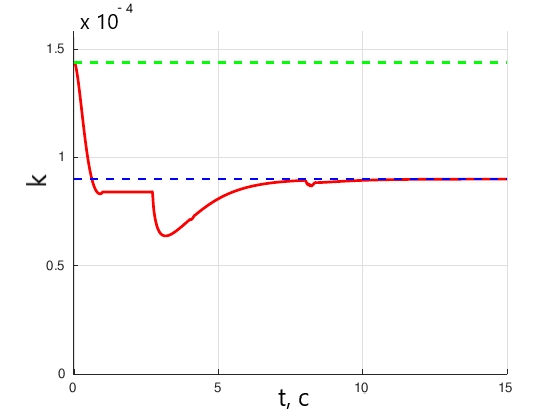
\includegraphics[clip,width=0.44\columnwidth]{k}%
	}
	\quad
	\subfloat[Оценка аэродинамического коэффициента пропеллера $b$]{%
		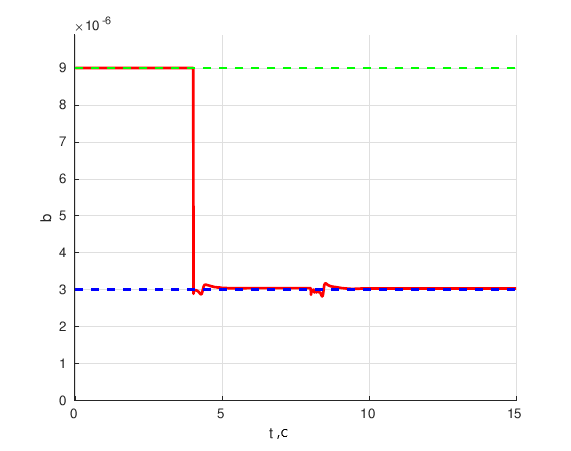
\includegraphics[clip,width=0.44\columnwidth]{b}%
	}
	\caption{ -- Уточнение параметров динамики БЛА}
	\label{fig:observer_k_b}
\end{figure}

	\chapter{Численные эксперименты}
\label{experiments_chapter}

\section{Структура модели}

Для подтверждения работоспособности синтезированной системы управления разработанные алгоритмы были реализованы в прикладном пакете Matlab Simulink.
В качестве численных методов для моделирования движения БЛА используется метод Рунге-Кутты 4-го порядка.

\section{Параметры управляемой динамики БЛА}

В данной работе, с учетом сформулированных в разделе \ref{section_ctrl_task} задач управления, для эксперимента выбраны параметры (см. таб. \ref{tb:params_table})., соответствующие небольшому квадрокоптеру, способному нести на борту дополнительную нагрузку в виде камеры высокого разрешения.
\begin{table}[h!]
	\centering
	\caption{ -- Параметры модели}\label{tb:params_table} 
	\begin{tabular}{lcl}
		\hline
		Параметр & Обозначение & Значение  \\\hline
		Общая масса & $M$ & 2 кг  \\
		Тензор инерции корпуса & $\bm J_B$ & $diag(2,\ 2,\ 4)\cdot{10^{-2}}$ кг$\cdot$м$^2$  \\
		Тензор инерции ротора & $\bm J_R$ & $diag(2,\ 2,\ 1)\cdot{10^{-5}}$ кг$\cdot$м$^2$  \\
		Миделево сечение корпуса & $S_{\perp}$ & 0,12 м$^2$ \\
		Луч & $L$ & 0,25 м \\
		Аэродинамический коэффициент & $C$ & 1,05\\
		Аэродинамический коэффициент & $k$ & 1,13$\cdot 10^{-5}$ Н$\cdot$с$^2\cdot$рад$^{-2}$ \\		
		Аэродинамический коэффициент & $b$ & 1,5$\cdot 10^{-6}$ Н$\cdot$м$\cdot$с$^2\cdot$рад$^{-2}$ \\		
		Максимальные обороты & $\tilde \omega_{max}$ & 1140 рад/с \\		
		Максимальный угол & $\theta_{max}$ & ${\pi}/{3}$ рад \\
		\hline
	\end{tabular}
\end{table}

\section{Обеспечение обратных связей в контуре управления}

Для обеспечения обратных связей в контуре управления выбран сигма-точечный фильтр Калмана.
В качестве основы для моделирования показаний бортовых сенсоров использована реально существующая и популярная среди разработчиков мультироторных роботов бортовая система Xsens MTi-7 \cite{xsens01}.

\section{Эксперимент: наблюдение за подвижным объектом}

В эксперименте аппарат должен выполнить наблюдение за подвижным объектом, летя неподалеку от него и ориентируя камеру, установленную спереди, так, чтобы объект находился в центре полученного изображения.
Мы не рассматриваем вопрос построения траектории БЛА, считая ее определённой заранее.
Целевая траектория БЛА (пунктирная линия), траектория пролета БЛА и наблюдаемого объекта изображены на рисунке \ref{fig:mau_traj}.
\begin{figure}[H]
	\centering
	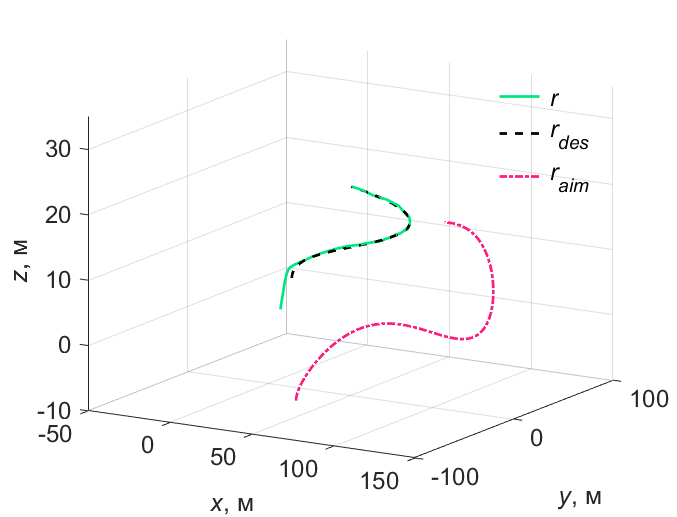
\includegraphics[width=14cm]{traj.png}
	\caption{ -- Траектории: целевая БЛА , пролета БЛА, наблюдаемого объекта}
	\label{fig:mau_traj}
\end{figure}
На рисунке \ref{fig:mau_errors}, слева изображены ошибки ориентации по углам крена, тангажа и рысканья, а справа -- ошибки положения квадрокоптера по осям $X$, $Y$ и $Z$.
Ошибки по каждому из углов ориентации после стабилизации не превышают пяти градусов.
После выхода аппарата на целевую кривую максимальное абсолютное отклонение от траектории составило чуть более полуметра.
\begin{figure}[h!]
	\centering
	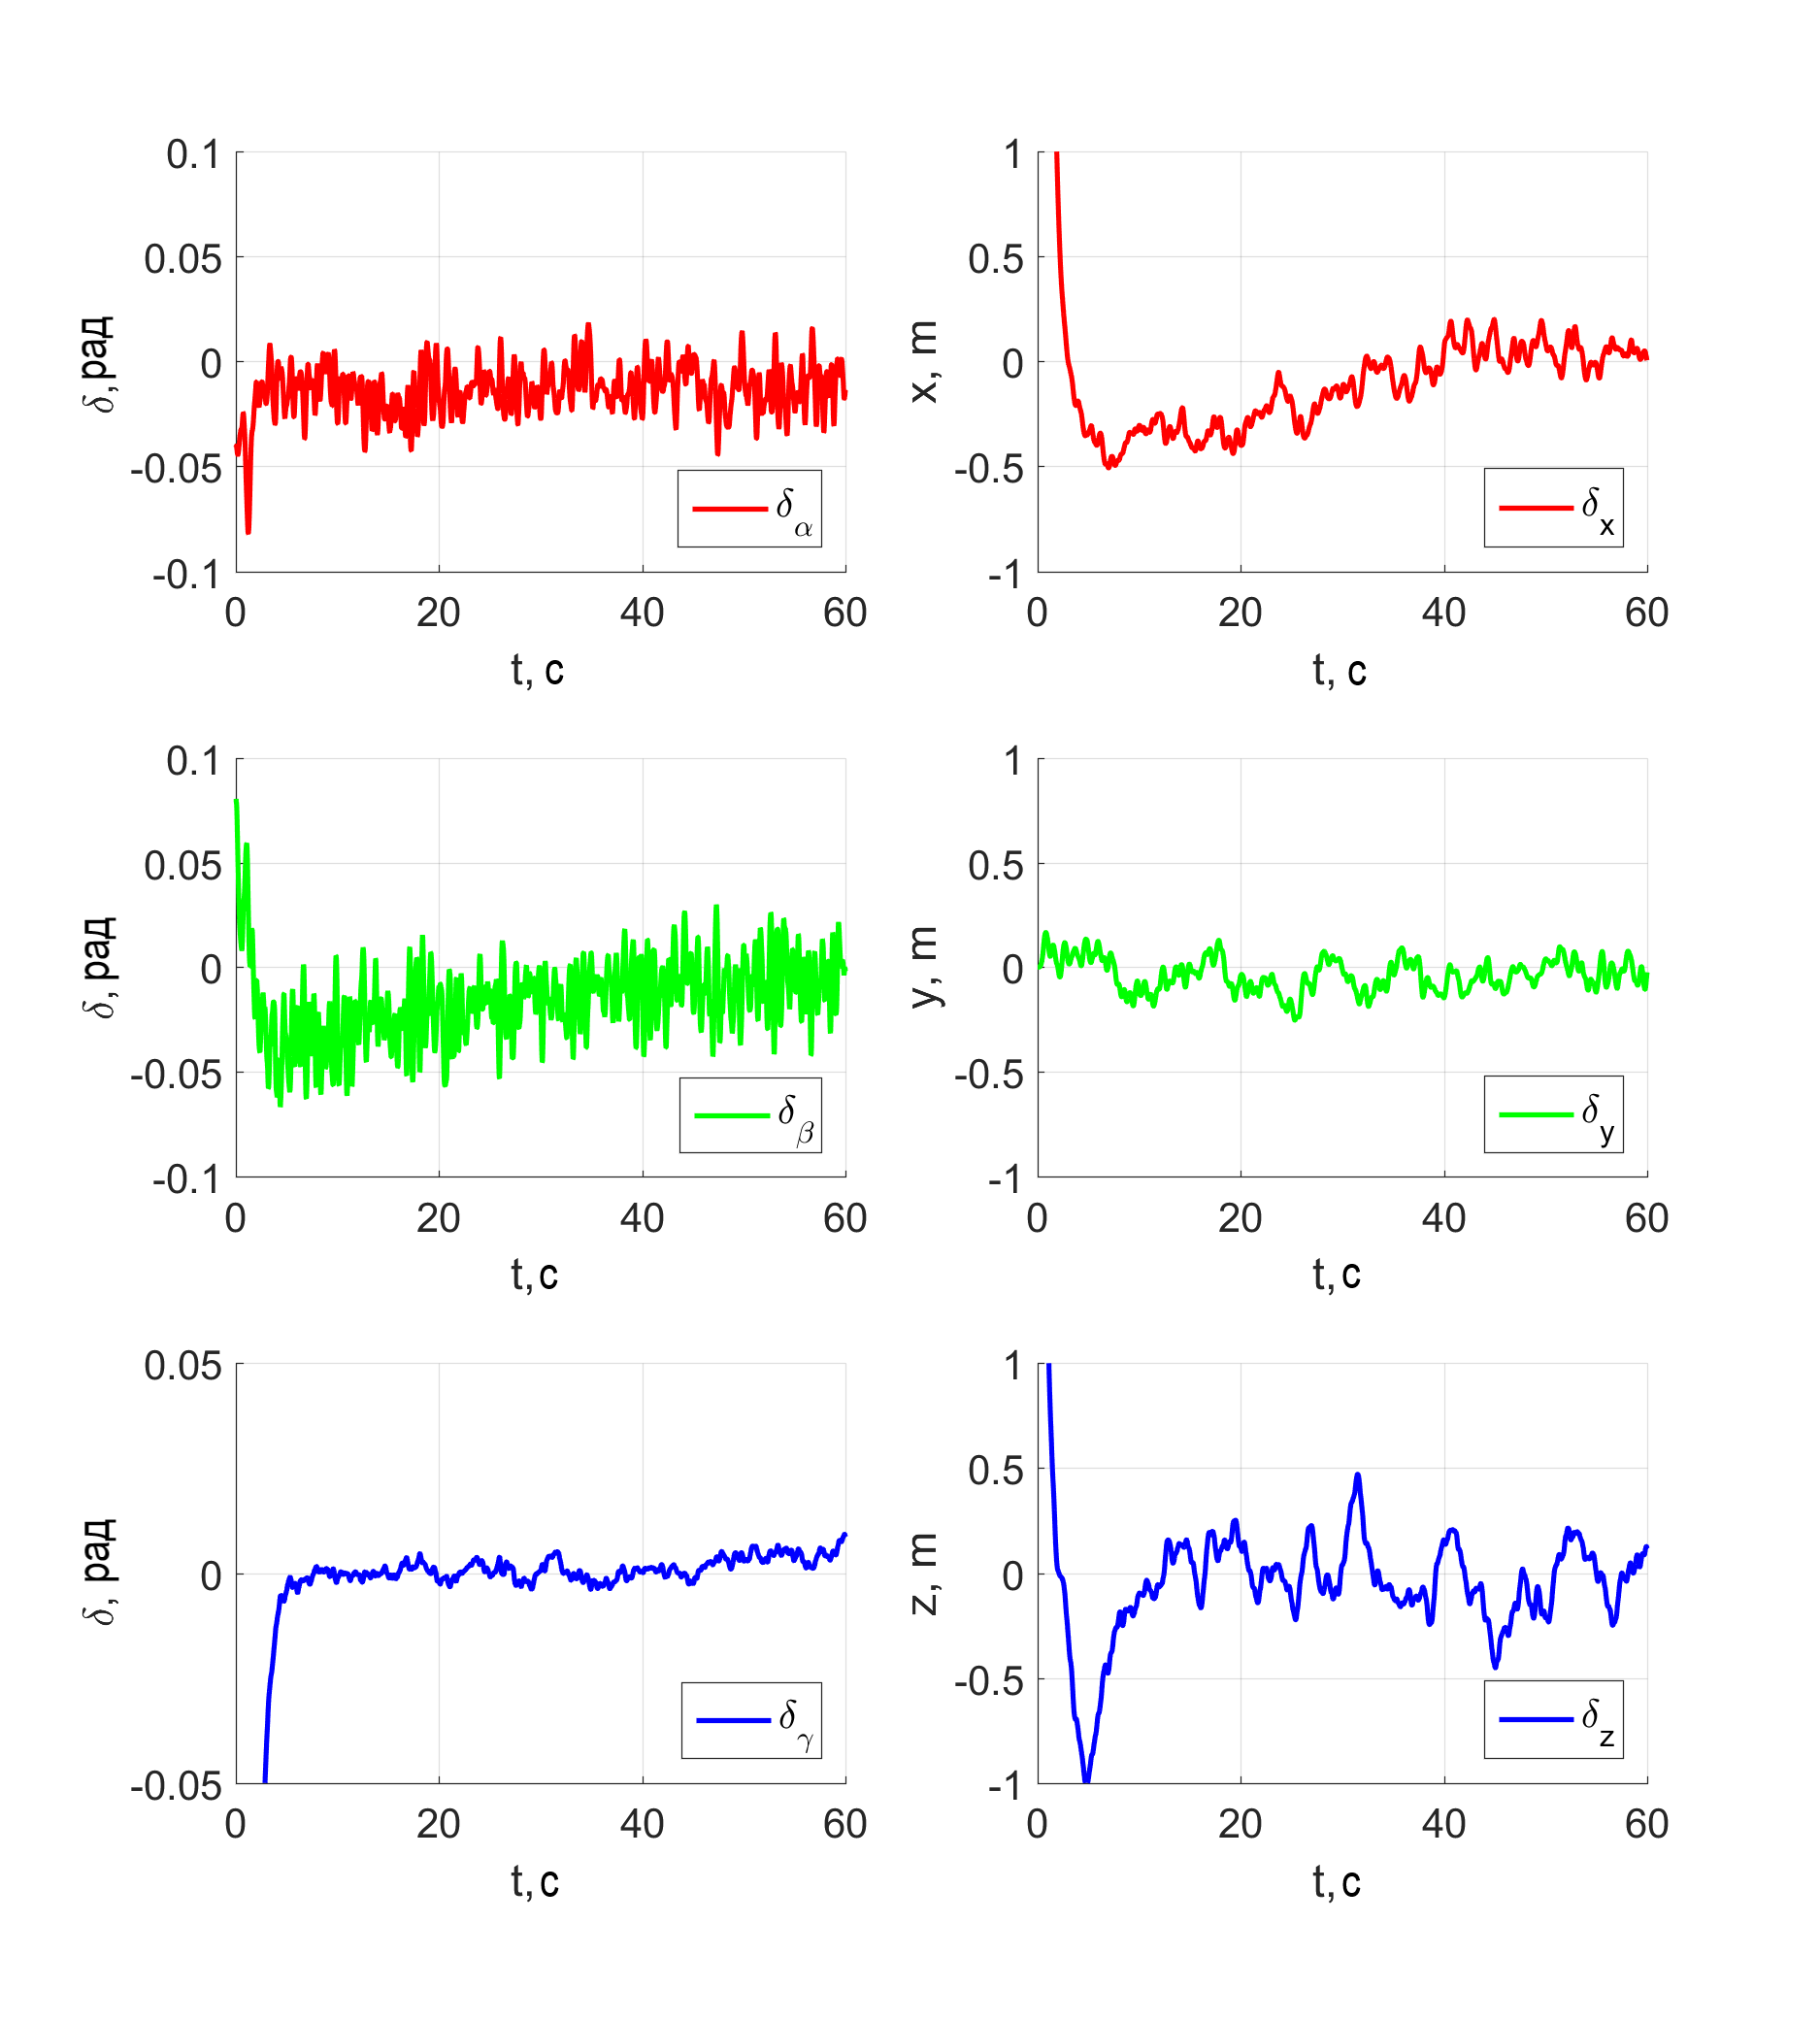
\includegraphics[width=16cm]{errors_rows.png}
	\caption{ -- Ошибка по ориентации и положению}
	\label{fig:mau_errors}
\end{figure}

На рисунке \ref{fig:mau_cam} можно проследить за траекторией наблюдаемого объекта на записи, которою можно сделать с помощью передней камеры.
Видно, что в начальный момент времени объект находится вне зоны видимости, затем перемещается в центр экрана и далее на протяжении всего времени манёвра ось визирования камеры отклоняется от направления на объект не более чем на 4 градуса.
\begin{figure}[h!]
	\centering
	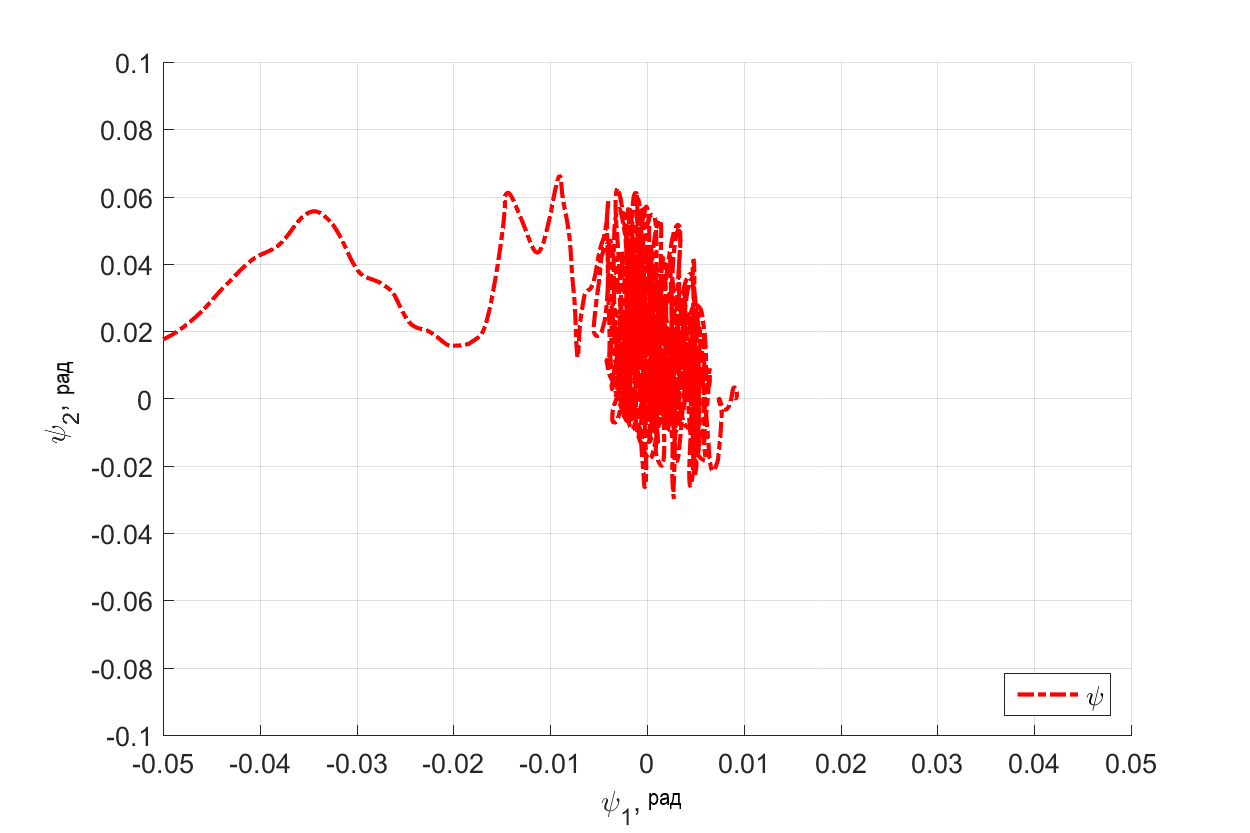
\includegraphics[width=16cm]{camera.png}
	\caption{ -- Траектория объекта на записи}
	\label{fig:mau_cam}
\end{figure}

В результате эксперимента мы оценили способность БЛА с поворотными роторами справляться со сложными маневрами, где необходимо независимо управлять ориентацией и положением аппарата.

\section{Эксперимент: экстренная посадка}

В данном эксперименте рассматривается сценарий отказа двух смежных двигателей. Применяются алгоритмы управления, описанные в разделе \ref{section_em_ctrl}. Как было отмечено, для возможности применения системы экстренного управления необходим значительный запас тяги двигателей и более широкие пределы отклонений сервоприводов. Поэтому в данном эксперименте параметры ограничений БЛА несколько отличаются от тех, что представлены в таблице \ref{tb:params_table}, а именно
\begin{equation}
\begin{aligned}
&\tilde{\omega}_{max} = 1318 \ \text{рад/c},
\\
&\theta_{max} = \pi.
\end{aligned}
\end{equation}

В начальный момент времени аппарат находится на высоте 25 метров недалеко от точки взлета.
При отказе двигателей начинается переход в режим экстренного управления.
За время менее 5 секунд высота БЛА упала более чем на 15 метров, но затем, когда аппарат стабилизировал свою ориентацию около целевых значений, падение прекратилось и аппарат приступил к плавному снижению со скоростью около 0,5 метров в секунду с одновременным движением в сторону места своего запуска.
На рисунке \ref{fig:em_coords} представлены параметры движения мультироторного робота в процессе экстренной посадки. Слева изображены графики компонент векторной части кватерниона ориентации корпуса, справа -- проекции координат центра масс БЛА на оси инерциальной системы отсчета.
\begin{figure}
	\centering
	\subfloat[крен]{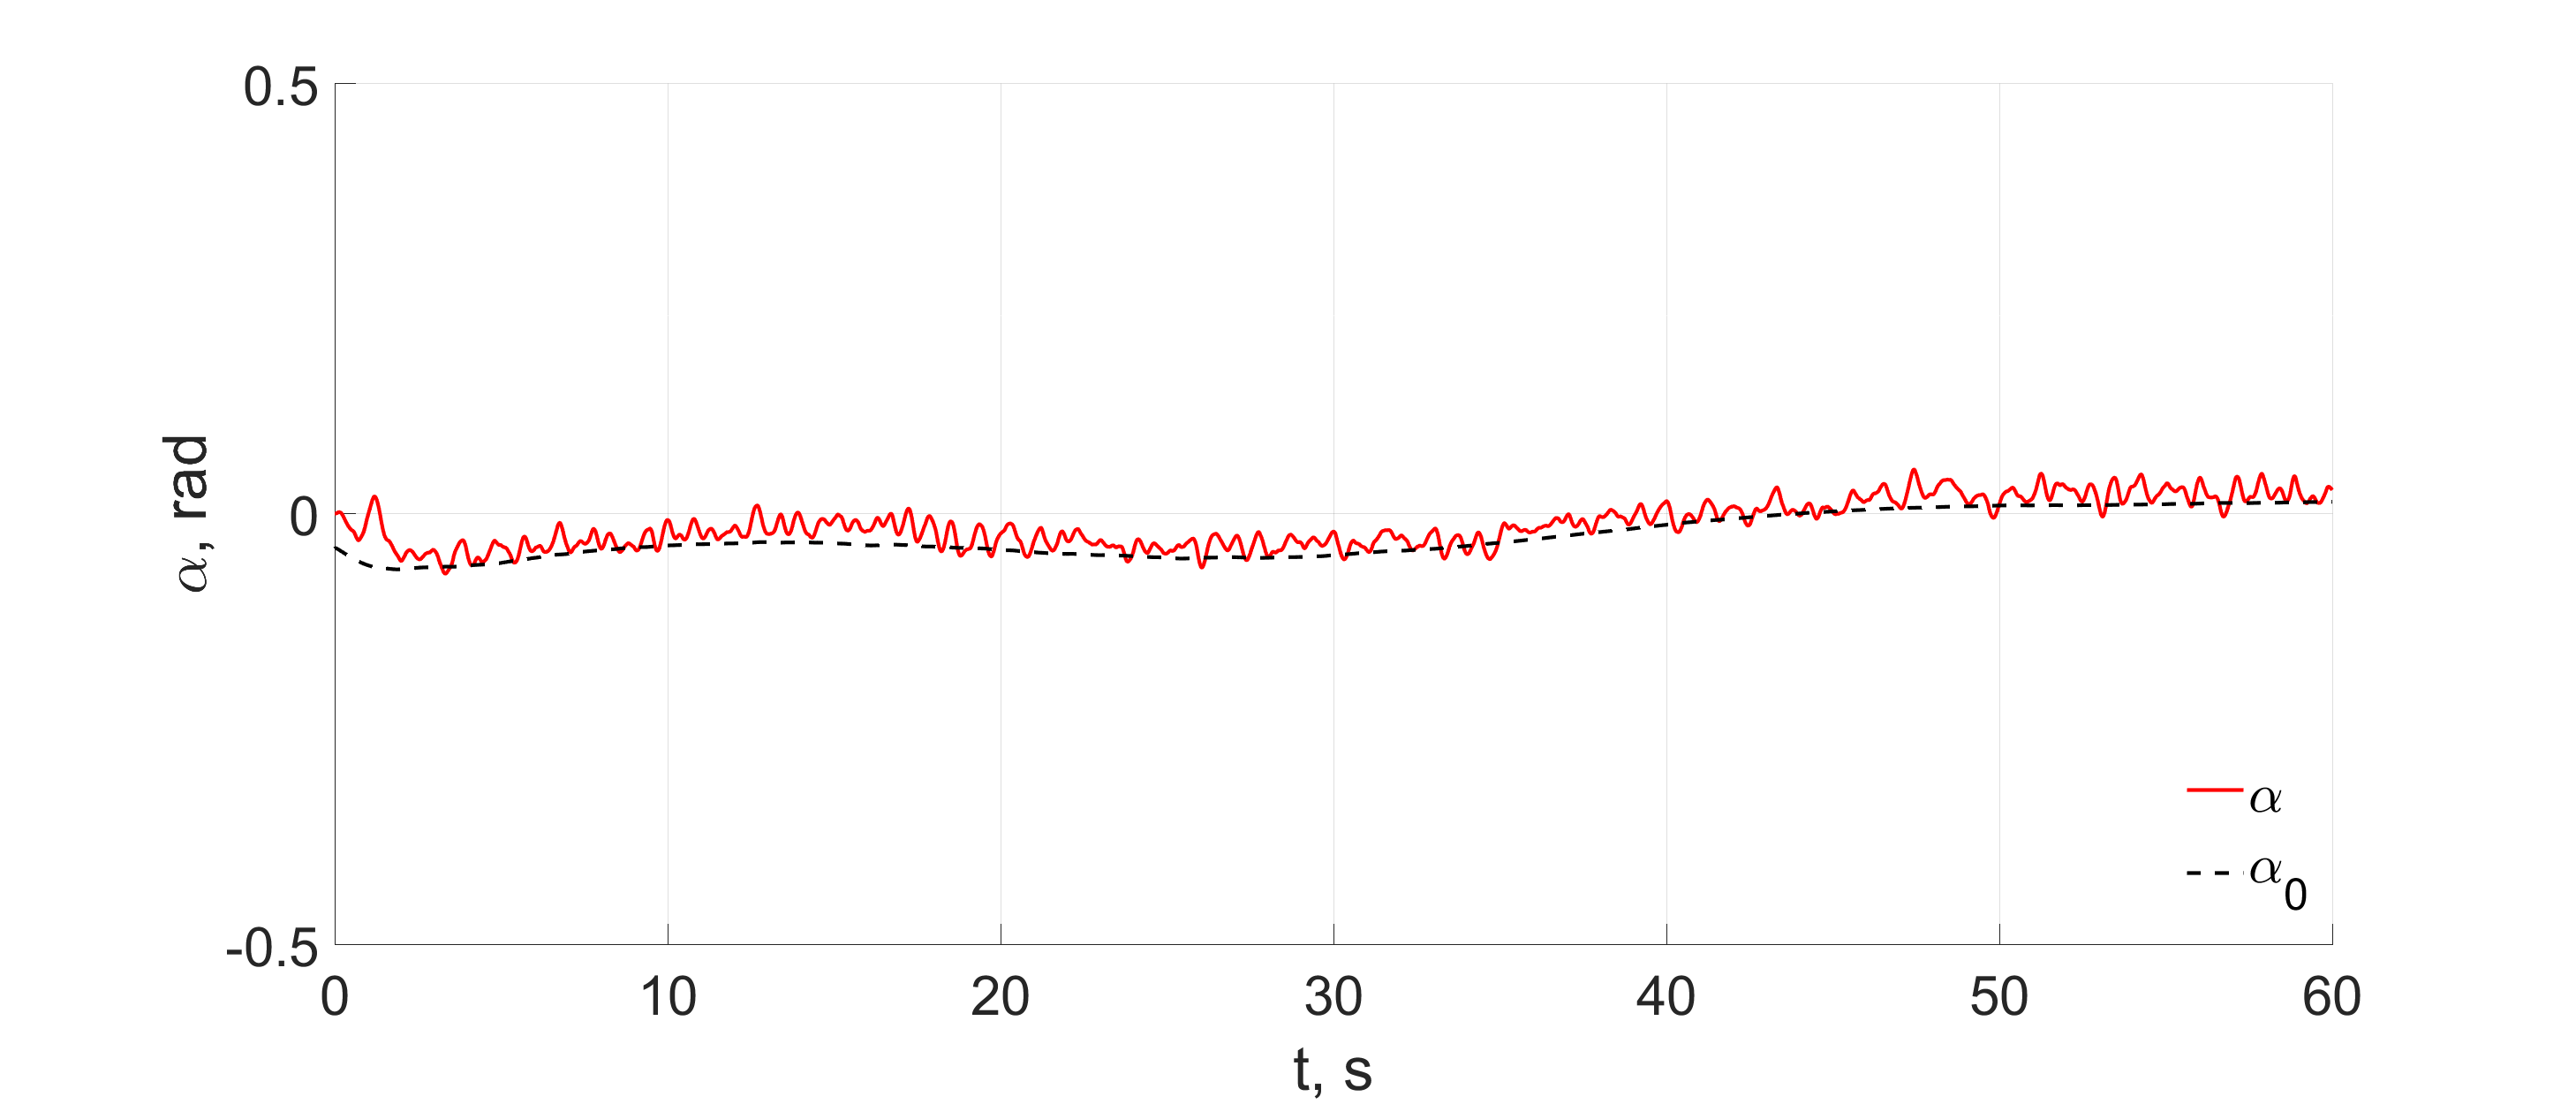
\includegraphics[width=8cm]{em/roll}}\hfil
	\subfloat[координата x]{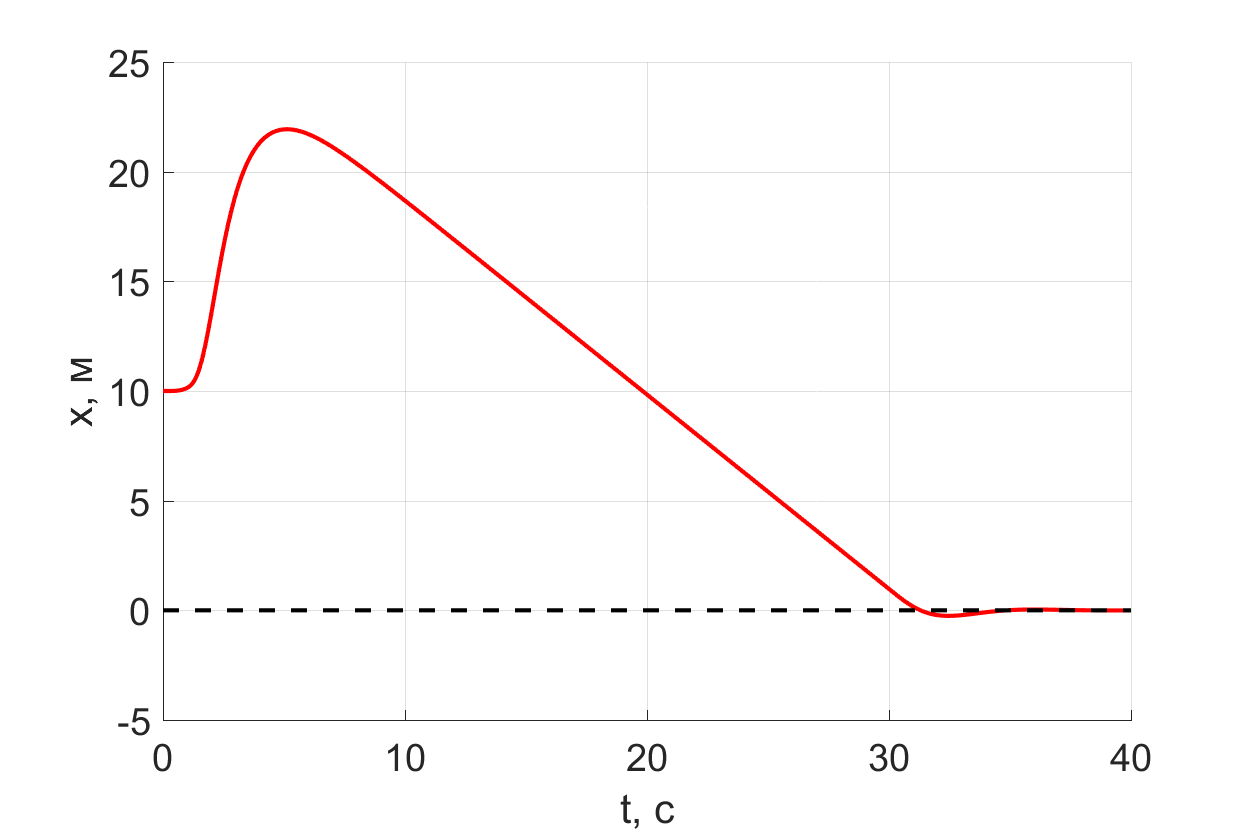
\includegraphics[width=8cm]{em/x}}
	
	\subfloat[тангаж]{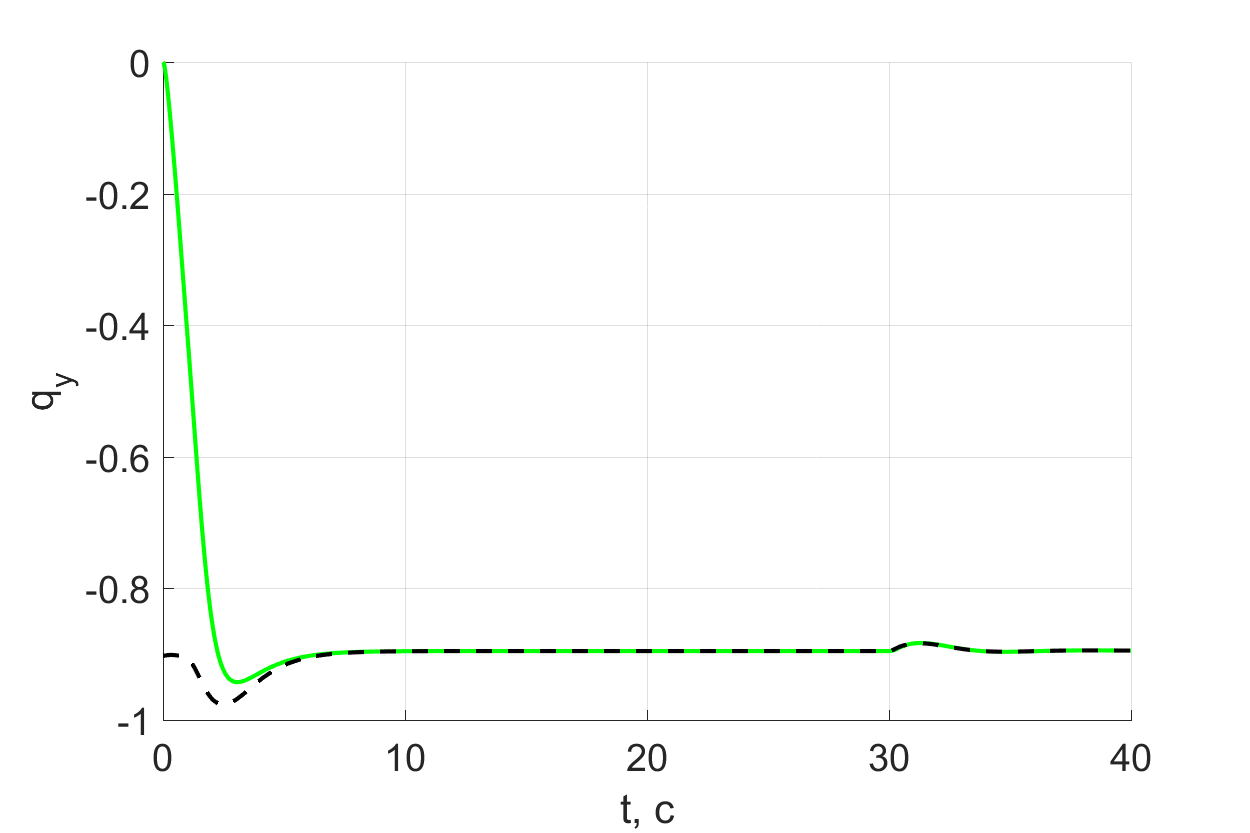
\includegraphics[width=8cm]{em/pitch}} \hfil 
	\subfloat[координата y]{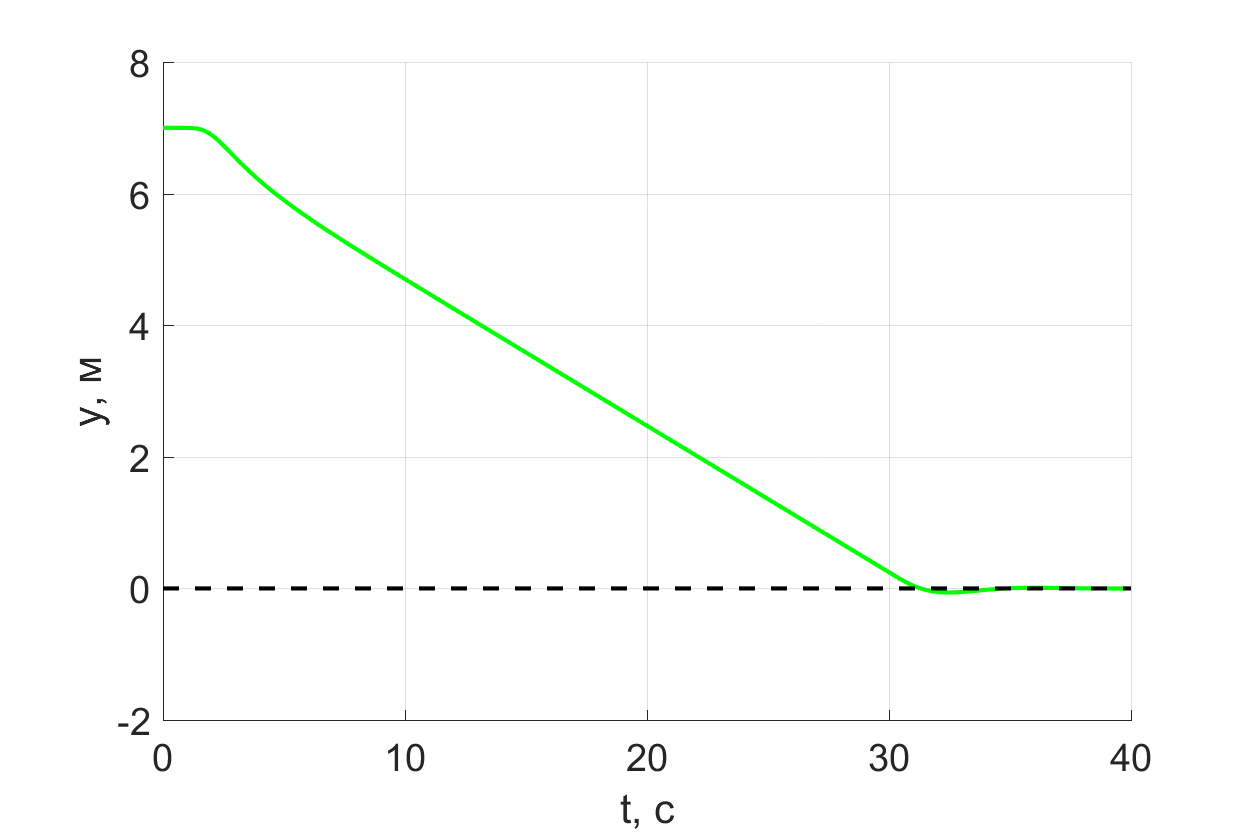
\includegraphics[width=8cm]{em/y}}  
	
	\subfloat[рысканье]{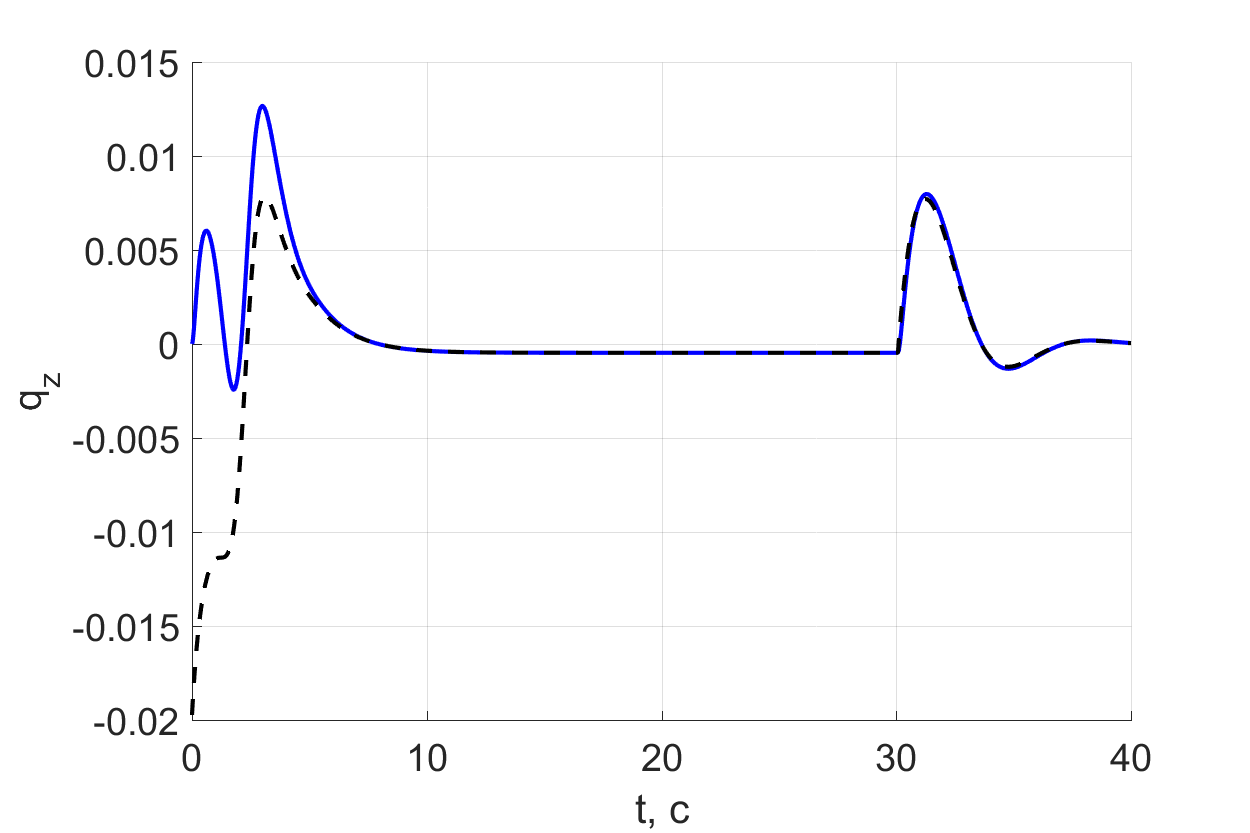
\includegraphics[width=8cm]{em/yaw}}\hfil
	\subfloat[координата z]{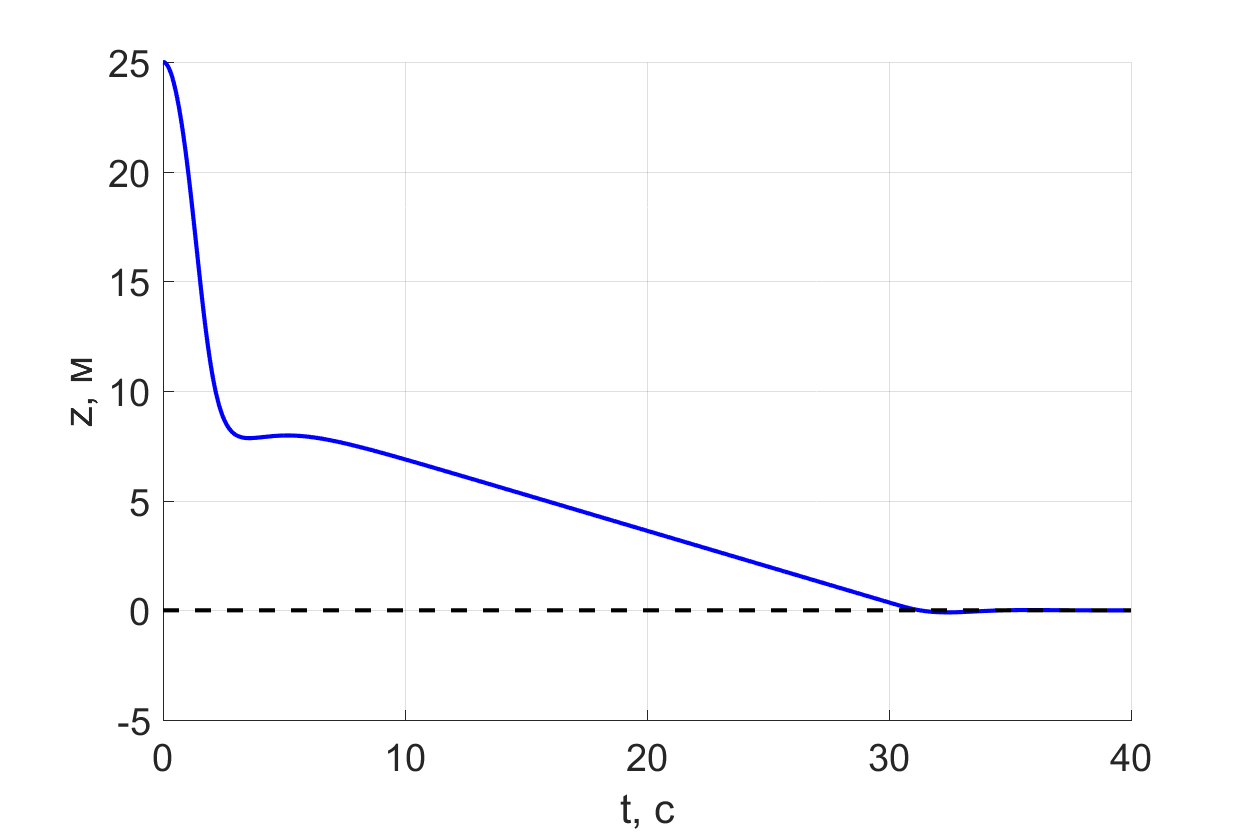
\includegraphics[width=8cm]{em/z}}
	\caption{ -- Параметры движения БЛА при экстренной посадке}
	\label{fig:em_coords}
\end{figure}
	\chapter{Заключение}
Основные результаты диссертации:
\begin{enumerate}
	\item Разработана математическая модель управляемой динамики квадрокоптера с поворотными роторами с учетом сил и моментов, действующих на все составные части системы;
	\item  Получено аналитическое решение задачи обратной динамики БЛА с поворотными роторами;
	\item Синтезирован контур управления квадрокоптером с поворотными роторами для независимого управления положением и ориентацией; 
	\item Разработан алгоритм для учета физических ограничений, накладываемых на исполнительные органы системы управления;
	\item Разработан алгоритм для идентификации основных параметров модели;
	\item Разработаны алгоритмы оценки состояния БЛА с поворотными роторами и проведен их сравнительный анализ.
	\item Разработаны алгоритмы экстренного управления квадрокоптером с поворотными роторами в случае отказа двух смежных двигателей.
\end{enumerate}
По результатам проведенного исследования можно сделать следующие
выводы:
\begin{enumerate}
	\item Расширение размерности вектора управляющих воздействий за счет применения сервоприводов, с помощью которых можно изменять направления тяги каждого из двигателей квадрокоптера, позволяет добиться независимого управления положением и ориентацией БЛА;
	\item Наличие аналитического решения задачи обратной динамики БЛА с поворотными роторами  позволяет ограничить каждую из компонент вектора управляющих воздействий с учетом технических возможностей исполнительных механизмов системы управления, что отражается на маневренных качествах БЛА;
	\item Конструкция квадрокоптера с поворотными роторами позволяет продолжить полет или осуществить безопасную посадку в случае выхода из строя одного или любой пары двигателей;
	\item Квадрокоптер с поворотными роторами способен выполнять задачу преследования подвижного объекта с его одновременным наблюдением с помощью жестко закрепленной на борту камеры.
\end{enumerate}
Таким образом, цели исследования, поставленные в диссертационной работе, достигнуты, и все
поставленные задачи – решены.
	\chapter{Список работ автора}
\begin{enumerate}
	\item Шавин М. Ю. Динамика БПЛА с поворотными роторами // Всероссийская конференция молодых учёных-механиков: Тезисы докладов (5 - 15 сентября 2017 г., г. Сочи, "Буревестник" МГУ)  – М.: МГУ, 2017. с N-M. ISBN 978-5-19-011217-7
	
	\item Притыкин Д.А., Шавин М.Ю., Гильманов Х.Г. Управляемая динамика квадрокоптера с поворотными роторами // Международная научная конференция Фундаментальные и прикладные задачи механики: Тезисы докладов (24 - 27 октября 2017 г., г. Москва) / М.: Издательство МГТУ им. Н.Э. Баумана, 2017. с 94-95.
	ISBN 978-5-7038-4800-5
	
	\item Шавин М. Ю. Управляемая динамика беспилотного летательного аппарата (БПЛА) с поворотными роторами // Труды 60-й Всероссийской научной конференции МФТИ. Аэрокосмические технологии. Секция теоретической механики. (20–26 ноября 2017 г., г. Долгопрудный) -- М.: МФТИ, 2017. с 79. ISBN 978-5-7417-0646-6
	
	\item Шавин М. Ю. Управление беспилотным летательным аппаратом (БПЛА) с поворотными роторами // Труды 60-й Всероссийской научной конференции МФТИ. Аэрокосмические технологии. Секция управления динамическими системами. (20–26 ноября 2017 г., г. Долгопрудный) -- М.: МФТИ, 2017. с 23-24. ISBN 978-5-7417-0646-6
	
	\item Шавин, М. Ю. Управляемая динамика квадрокоптера с поворотными роторами. Инженерный журнал: наука и инновации, 2018, 76 (4), doi: 10.18698/ 2308-6033-2018-4-1755.
	
	\item Mikhail Yu. Shavin. Dynamics and Control of UAV with Variable Geometry // The Seventh International Conference “Geometry, Dynamics, Integrable Systems” – GDIS 2018: Book of Abstracts. (June 5-9, 2018, Moscow Institute of Physics and Technology, Moscow (Dolgoprudniy)) – Moscow – Izhevsk: Publishing Center “Institute of Computer Science”, 2018. pp. 91-93. ISBN 975-5-4344-0520-1
	
	\item Shavin M. Design and identification of tilt-motor quadrotor control system. // The 14th International Conference on vibration engineering and technology of machinery (VETOMAC XIV): Book of Abstracts (September 10 - 13), 2018, Lisbon, Portugal.
	
	\item Mikhail Shavin. Design and identification of tilt-motor quadrotor control system 
	// MATEC Web of Conferences 211, 02013 (2018) VETOMAC XIV
	MATEC Web Conf. Volume 211, 2018 The 14th International Conference on Vibration Engineering and Technology of Machinery (VETOMAC XIV). 10 October 2018
	
	\item Шавин М., Притыкин Д. Управляемая динамика квадрокоптера с поворотными роторами: алгоритмы оценки состояния // Проблемы механики и управления: Материалы международной конференции (16 - 22 сентября 2018 г., г. Махачкала) / ред. И.Г. Горячева – М.: Издательство Московского университета, 2018. с 337-339
\end{enumerate}
	\chapter{Приложение}

Выражения для функций, входящих в уравнения обращенной динамики БЛА с поворотными роторами:
\begin{equation}
A_1 = (F_3kl + bF_2 - kT_2); \label{eq:app_solve_AB_begin}
\end{equation}
\begin{equation}
A_2 = (F_3kl + bF_1 + kT_1);
\end{equation}
\begin{equation}
A_3 = (F_3kl - bF_2 + kT_2);
\end{equation}
\begin{equation}
A_4 = (F_3kl - bF_1 - kT_1);
\end{equation}
\begin{equation}
B_1 = (bF_3 - kT_3 - F_2kl);
\end{equation}
\begin{equation}
B_2 = (bF_3 + kT_3 - F_1kl);
\end{equation}
\begin{equation}
B_3 = (bF_3 - kT_3 + F_2kl);
\end{equation}
\begin{equation}
B_4 = (bF_3 + kT_3 + F_1kl). \label{eq:app_solve_AB_end}
\end{equation}

Выражения для компонент вектора управляющих воздействий для обращенной динамики БЛА с двумя работающими двигателями: 

\begin{equation} \label{eq:app_em_solve_begin}
\begin{aligned}
&\tilde \omega_1 = \\&-\Big[2b^4F_1^2 + 4b^3F_1kT_2 + 4b^2F_1^2k^2l^2 - 2\sqrt{2}b^2F_1k^2lT_3 + 2b^2k^2T_2^2 + 4bF_1k^3l^2T_2 -\\ &-2\sqrt{2}bk^3lT_2T_3 + 2F_1^2k^4l^4 - 2\sqrt{2}F_1k^4l^3T_3 + 2k^4l^2T_1^2 - 4k^4l^2T_1T_2 + 2k^4l^2T_2^2 +\\ &+k^4l^2T_3^2 \Big]^{(0.5)} \Big(2k^2l(b^2 + k^2l^2)^{0.5)}\Big)^{-1};
\end{aligned}
\end{equation}

\begin{equation}
\begin{aligned}
&\tilde \omega_4 = \\&\Big[2b^4F_1^2 + 4b^3F_1kT_2 + 4b^2F_1^2k^2l^2 + 2\sqrt{2}b^2F_1k^2lT_3 + 2b^2k^2T_2^2 + 4bF_1k^3l^2T_2 + \\& +2\sqrt{2}bk^3lT_2T_3 + 2F_1^2k^4l^4 + 2\sqrt{2}F_1k^4l^3T_3 + 2k^4l^2T_1^2 + 4k^4l^2T_1T_2 + 2k^4l^2T_2^2 + \\& +k^4l^2T_3^2\Big]^{0.5} \Big(2k^2l(b^2 + k^2l^2)^{0.5}\Big)^{-1};
\end{aligned}
\end{equation}

\begin{equation}
\begin{aligned}
&\tilde \theta_1 = \\&2\text{arctg} \Big[\Big(2b^3F_1 - 2k^3l^2T_1 + 2k^3l^2T_2 + \sqrt{2}(b^2 + k^2l^2)^{0.5}
(2b^4F_1^2 + 4b^3F_1kT_2 +\\&+ 4b^2F_1^2k^2l^2 - 2\sqrt{2}b^2F_1k^2lT_3 + 2b^2k^2T_2^2 + 4bF_1k^3l^2T_2 - 2\sqrt{2}bk^3lT_2T_3 + 2F_1^2k^4l^4 - \\ -&2\sqrt{2}F_1k^4l^3T_3 + 2k^4l^2T_1^2 - 4k^4l^2T_1T_2 + 2k^4l^2T_2^2 + k^4l^2T_3^2)^{0.5} + 2b^2kT_2 + 2bF_1k^2l^2 - \\& -\sqrt{2}bk^2lT_3 \Big) \Big(kl(2F_1b^2 + 2T_1bk + 2F_1k^2l^2 - \sqrt{2}T_3k^2l)\Big)^{-1}\Big];
\end{aligned}
\end{equation}

\begin{equation} \label{eq:app_em_solve_end}
\begin{aligned}
&\tilde \theta_4 = \\&-2\text{arctg}\Big[\Big(2b^3F_1 + 2k^3l^2T_1 + 2k^3l^2T_2 + \sqrt{2}(b^2 + k^2l^2)^{0.5}(2b^4F_1^2 +  4b^3F_1kT_2  +\\& +4b^2F_1^2k^2l^2 + 2\sqrt{2}b^2F_1k^2lT_3 + 2b^2k^2T_2^2 + 4bF_1k^3l^2T_2 + 2\sqrt{2}bk^3lT_2T_3 + 2F_1^2k^4l^4 + \\& +2\sqrt{2}F_1k^4l^3T_3 + 2k^4l^2T_1^2 + 4k^4l^2T_1T_2 + 2k^4l^2T_2^2 + k^4l^2T_3^2)^{0.5} + 2b^2kT_2 + \\&+2bF_1k^2l^2 +\sqrt{2}bk^2lT_3\Big)\Big(kl(2F_1b^2 - 2T_1bk + 2F_1k^2l^2 + \sqrt{2}T_3k^2l)\Big)^{-1}\Big].
\end{aligned}
\end{equation}



	\sloppy
	\printbibliography
\end{document}


